\documentclass[a4paper]{book}
\usepackage[utf8]{inputenc}
\usepackage{graphicx}
\usepackage[T1]{fontenc} 
\usepackage[spanish]{babel}
\usepackage{titlesec}
\usepackage{geometry}
\usepackage{amsmath}
\usepackage{float}
\usepackage{verbatim}
\usepackage{booktabs}
\usepackage{colortbl}
\usepackage[table]{xcolor}
\usepackage{array}
\usepackage{tabularx}
\usepackage{hyperref}
\usepackage{fancyhdr}
\usepackage{lipsum}


\hypersetup{
    colorlinks=true,
    linkcolor=blue,
    urlcolor=blue,
    filecolor=magenta,      
    citecolor=blue,
    pdftitle={SafeSight - Proyecto Argos},
    pdfauthor={Edwin Benito Castillo Hernández, David de Jesús Hernández Hernández, Alfonso Oropeza Sangabriel, Erick Rivas Esquivel},
    %bookmarks=true,
    pdfpagemode=FullScreen,
}

\titleformat{\chapter}[display]
  {\normalfont\huge\bfseries}{\chaptertitlename\ \thechapter}{20pt}{\Huge}
\titlespacing*{\chapter}{0pt}{-30pt}{20pt}

\let\cleardoublepage\clearpage

\setcounter{secnumdepth}{3}
\setcounter{tocdepth}{3}

\begin{document}


\begin{titlepage}
    \centering

    
\includegraphics[width=0.3\textwidth]{logo_upp.jpg}\par

    \vspace{1cm}
    {\Huge\bfseries Universidad Politécnica de Pachuca\par}
    \vspace{2cm}

    {\Large\bfseries SafeSight\par}
    \vspace{1cm}

    {\Huge\bfseries Proyecto Argos\par}
    \vspace{1.5cm}

    {\Large Ingeniería en Tecnologías de la Información e Innovación Digital\par}
    \vspace{1cm}

    {\large\bfseries Integrantes:\par}
    \vspace{0.5cm}
    {\large Castillo Hernández Edwin Benito -- 2431124902\par}
    {\large Hernández Hernández David de Jesús -- 2431124979\par}
    {\large Oropeza Sangabriel Alfonso -- 2431124918\par}
    {\large Rivas Esquivel Erick -- 2431124895\par}
    \vspace{0.5cm}

    {\large\bfseries PROYECTO INTEGRADOR I\par}
    {\large\bfseries TÓPICOS DE CALIDAD PARA EL DISEÑO DE SOFTWARE\par}
    {\large\bfseries DESARROLLO DEL PENSAMIENTO Y TOMA DE DECISIONES\par}
    
    \vspace{1cm}

    {\large Mayo-agosto 2025\par}
    \vfill

    \thispagestyle{empty}
\end{titlepage}







\frontmatter
\tableofcontents

\mainmatter
\clearpage
\chapter{Perfil de Proyecto}

\section{Identificación y Análisis del Problema}




En la Universidad Politécnica de Pachuca, el registro de entrada y asistencia provoca saturación en los accesos debido a procesos manuales y falta de tecnología adecuada. Esta situación genera retrasos para los alumnos, dificulta el inicio puntual de las clases y complica el registro para los padres, afectando la convivencia y el orden institucional.

La acumulación de personas en los puntos de acceso impacta la dinámica diaria y la experiencia de la comunidad universitaria.


%\clearpage
\section{Objetivos del Proyecto}

\subsection{Objetivo General}


Establecer un sistema de control eficiente de usuarios en la Universidad Politécnica de Pachuca con el fin de garantizar la seguridad, el registro automatizado de accesos y la trazabilidad de la asistencia escolar.

\subsection{Objetivos Específicos}

\begin{itemize}
    \item Implementar un mecanismo de reconocimiento facial que registre la entrada del alumnado a la institución educativa.
    \item Proporcionar a los docentes una herramienta digital para verificar la asistencia de los estudiantes a sus respectivas clases.
    \item Desarrollar una plataforma en línea que permita a los padres de familia consultar en tiempo real la asistencia de sus hijos tanto al plantel como a sus clases programadas.
    \item Restringir el acceso a personas no autorizadas, reforzando la seguridad del entorno escolar mediante validaciones tecnológicas.
\end{itemize}

\clearpage
\section{Necesidades Tecnológicas}

El sistema Argos requiere infraestructura tecnológica adecuada: dispositivos biométricos, redes confiables, servidores y plataformas digitales. Estos recursos permiten automatizar procesos y proteger la información.

La siguiente imagen muestra el esquema básico de la solución tecnológica propuesta.
\subsection{Mapa Mental}

\begin{figure}[H]
    \centering
    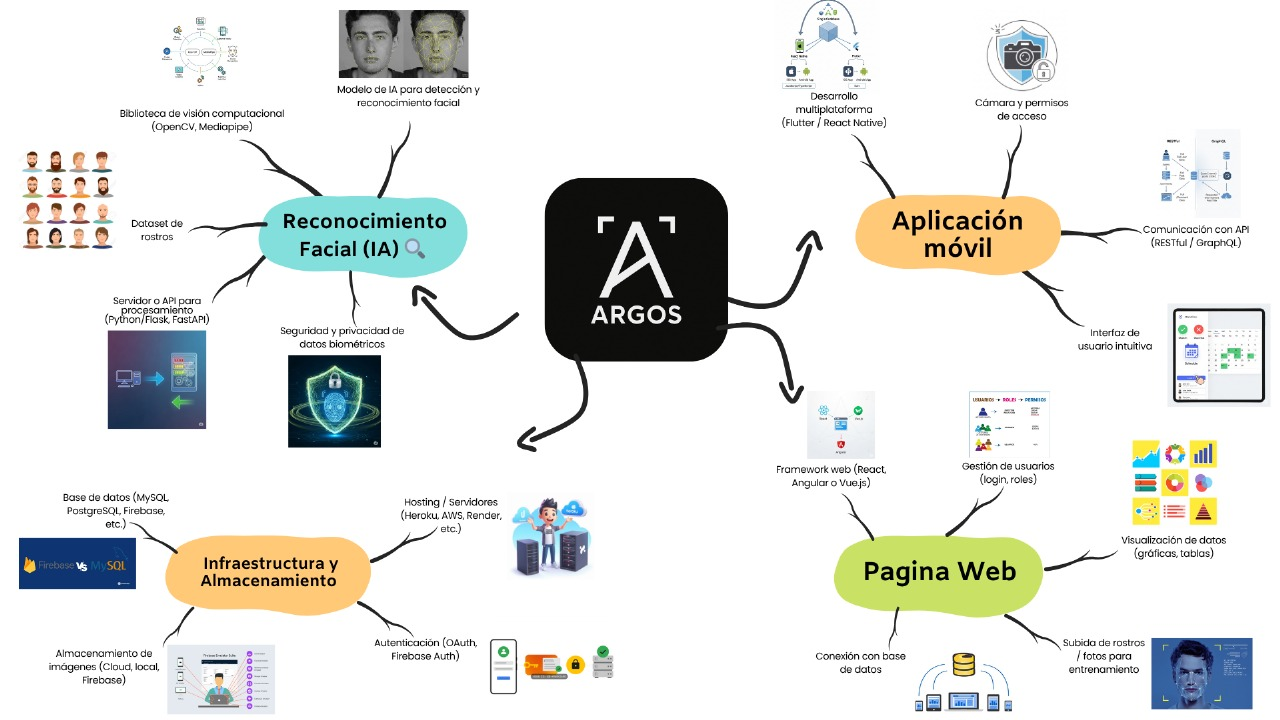
\includegraphics[width=1.0\textwidth]{./Media/mapaArgos.jpg}
    \caption{Mapa general de la infraestructura tecnológica propuesta para Argos}
    \label{fig:infraestructura}
\end{figure}

\clearpage
\section{Evaluación de Condiciones y Necesidades del Proyecto}

\subsection{Técnicas para identificar problemas}

La identificación de problemas es un paso fundamental en el desarrollo de un proyecto, esto permite comprender las necesidades 
reales del contexto, los usuarios y las organizaciones involucradas. A continuación, se describen las técnicas básicas 
utilizadas en esta etapa: Estas técnicas fueron seleccionadas considerando la diversidad de actores involucrados 
(alumnos, personal administrativo, padres de familia, docentes) y la complejidad del sistema propuesto.

\subsubsection*{Análisis de Cuestionarios y Entrevistas}
Durante el mes de junio se aplicaron encuestas y entrevistas presenciales en las instalaciones de la
 Universidad Politécnica de Pachuca, principalmente en horarios de entrada y salida escolar. El objetivo de esta técnica 
 fue identificar necesidades, dificultades y expectativas de los usuarios clave respecto al sistema propuesto. 
 Su utilidad radica en que permitió obtener información directa y variada de alumnos, docentes y personal administrativo, 
 facilitando la detección de problemas y oportunidades de mejora.

\subsubsection*{Observación Directa}
Esta técnica se llevó a cabo durante junio en los accesos principales de la institución, en los horarios de mayor afluencia. 
El objetivo fue analizar el comportamiento real de los usuarios y los procesos actuales de registro de entrada.
 La observación directa resultó útil para detectar problemas no expresados verbalmente y observar el flujo real de personas y 
 los tiempos de espera.

\subsubsection*{Consulta con Expertos}
Durante el mes de junio se realizaron reuniones presenciales y virtuales con especialistas en tecnologías de la información 
y gestión escolar. El objetivo fue validar la viabilidad técnica y operativa de la solución propuesta. 
Esta técnica fue útil porque aportó recomendaciones sobre integración tecnológica, seguridad y
 mejores prácticas, anticipando posibles retos y permitiendo ajustar el diseño conceptual del sistema.





% Para que las subsubsecciones aparezcan numeradas y en el índice
\setcounter{secnumdepth}{3}
\setcounter{tocdepth}{3}


\clearpage

\subsection{Método Delphi}

El método \textbf{Delphi} es una técnica de pronóstico que busca el consenso de un grupo de expertos. Se basa en rondas de cuestionarios anónimos, donde la retroalimentación gradual converge hacia un acuerdo. Para el desarrollo del proyecto \textbf{Argos}, la empresa \textbf{SafeSight} aplicó este método para evaluar y refinar la propuesta de sistema de control de acceso escolar con reconocimiento facial, asegurando una solución robusta y adaptada a la comunidad educativa.

\begin{figure}[H]
    \centering
    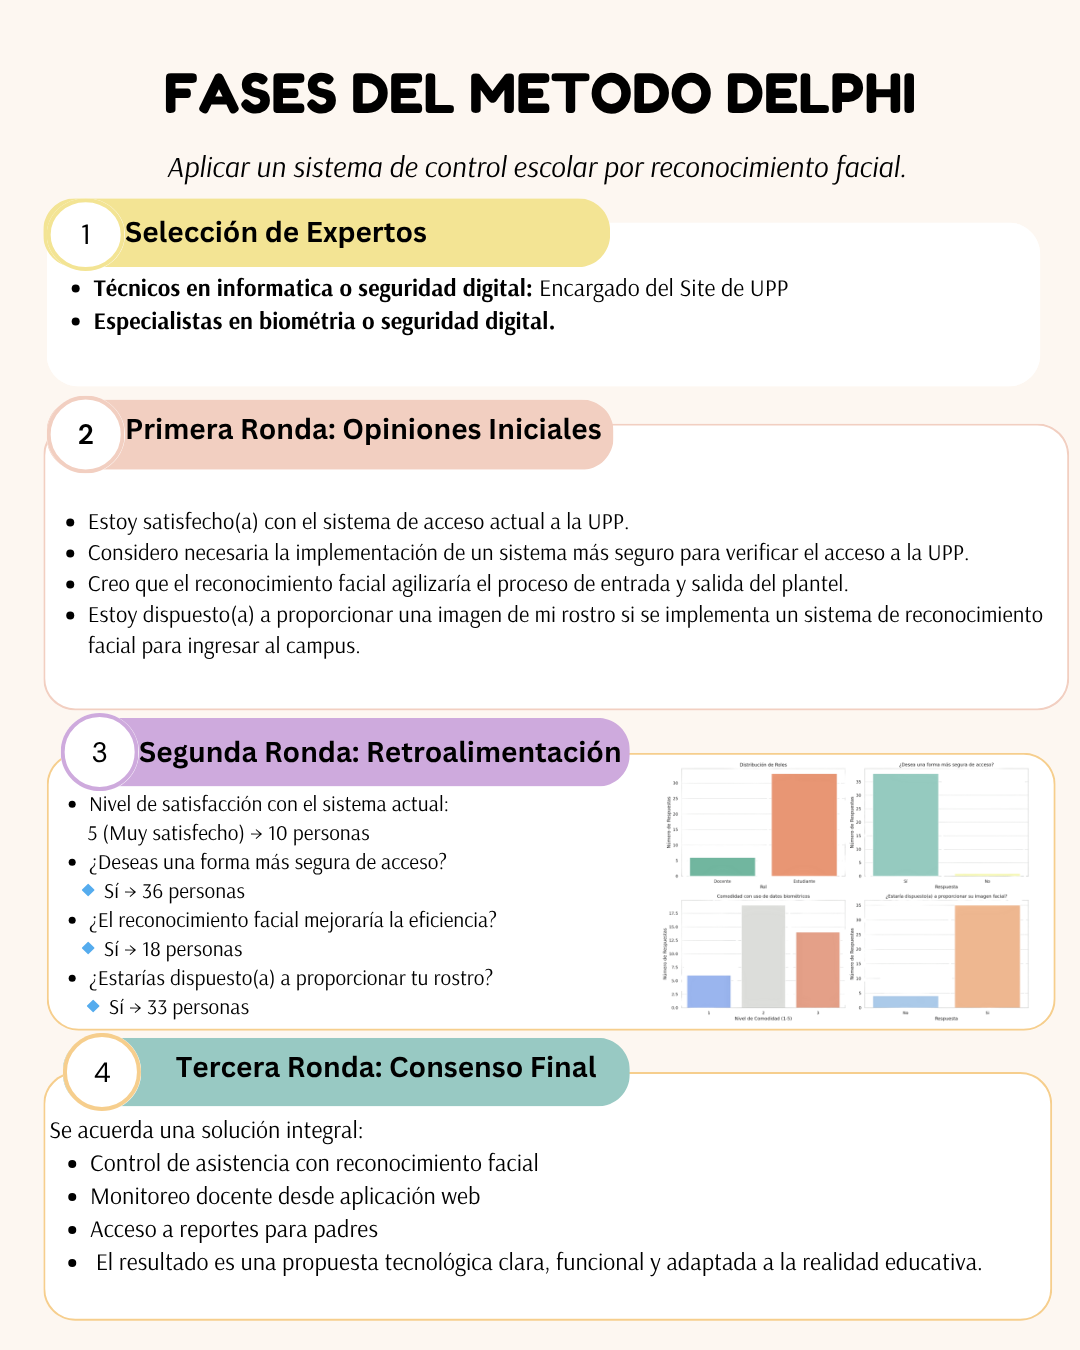
\includegraphics[width=0.85\textwidth]{./Media/Delphi.png}
    \caption{Ejemplo de aplicación del Método Delphi por SafeSight para el proyecto Argos}
    \label{fig:delphi}
\end{figure}

\clearpage
\section{Visión del Proyecto}

El proyecto Argos busca modernizar el acceso y la asistencia escolar en la Universidad Politécnica de Pachuca con un sistema automatizado, seguro y eficiente. A corto plazo, reducirá los tiempos de acceso y errores en el registro; a mediano, mejorará la comunicación y el monitoreo de asistencia; y a largo plazo, consolidará un entorno escolar innovador y confiable. Argos fortalecerá la confianza, la puntualidad y la toma de decisiones, y servirá como modelo para otras instituciones educativas.

Además, Argos impulsará el desarrollo de competencias digitales en la comunidad escolar y facilitará la adaptación a nuevas tecnologías, contribuyendo al crecimiento institucional y al bienestar de todos los usuarios involucrados.


%\clearpage
\section{Alcance del Proyecto}


El presente proyecto se enfoca en el análisis, planeación, diseño y pruebas de usabilidad de una solución para optimizar el control de acceso y la gestión de la asistencia en entornos educativos, tomando como referencia la Universidad Politécnica de Pachuca. La implementación de esta solución se plantea como un proyecto a largo plazo, con la intención de abordar las necesidades actuales y futuras de la institución educativa.


El proyecto no contempla el desarrollo ni la implementación de sistemas de seguridad física, como cámaras de vigilancia o alarmas, ni la integración con sistemas externos de control de acceso que no sean los mencionados. Asimismo, por el momento no contempla el reconocimiento facial como mecanismo de identificación.



%\clearpage
\section{Público Objetivo}


El público objetivo del proyecto está centrado en la Universidad Politécnica de Pachuca, e incluye a:

\begin{itemize}
\item Alumnos (usuarios finales)
\item Docentes
\item Visitantes
\item Personal administrativo (Secretaría, Control Escolar)
\item Dirección escolar / Rectoría
\item Proveedores de servicios
\item Personal de seguridad escolar
\item Padres de familia (beneficiarios indirectos)
\end{itemize}

\clearpage
\section{Recursos Disponibles}


Para la correcta ejecución y desarrollo del proyecto, se identificaron y organizaron los recursos disponibles en las siguientes categorías: humanos, materiales, tecnológicos y servicios. A continuación, se presentan las tablas correspondientes a cada tipo de recurso:

\subsection{Recursos Humanos}

% Recursos Humanos
\begin{table}[h!]
\centering
\footnotesize
\setlength{\tabcolsep}{3.5pt}
\renewcommand{\arraystretch}{0.98}
\begin{tabular}{|l|c|}
\hline
	extbf{Recurso Humano} & \textbf{Costo mensual (MXN)} \\
\hline
Líder de Proyecto Jr & \$25,000 \\
Analista Jr & \$20,000 \\
Diseñador UI/UX Jr & \$20,000 \\
Desarrollador de IA Jr & \$40,000 \\
Desarrollador Mobile Jr & \$36,000 \\
Desarrollador Backend Jr & \$35,000 \\
Desarrollador Frontend Jr & \$33,000 \\
QA Jr & \$18,000 \\
Administrador de Base de Datos Jr & \$22,000 \\
Especialista en Seguridad Jr & \$25,000 \\
Consultor en Reconocimiento Facial Jr & \$28,000 \\
\hline
	extbf{Total Recursos Humanos} & \textbf{\$302,000} \\
\hline
\end{tabular}
\caption{Recursos humanos y costos mensuales estimados}
\end{table}

\subsection{Recursos Materiales y Tecnológicos}

% Recursos Materiales y Tecnológicos
\begin{table}[h!]
\centering
\footnotesize
\setlength{\tabcolsep}{3.5pt}
\renewcommand{\arraystretch}{0.98}
\begin{tabular}{|l|c|}
\hline
\textbf{Recurso Material/Tecnológico} & \textbf{Costo mensual (MXN)} \\
\hline
Cámaras de reconocimiento facial (3 unidades) & \$3,000 \\
Servidores en la nube & \$2,500 \\
Licencias de software & \$1,200 \\
Internet y servicios de red & \$1,000 \\
Material de oficina y papelería & \$500 \\
\hline
\textbf{Total Material/Tecnológico} & \textbf{\$8,200} \\
\hline
\end{tabular}
\caption{Recursos materiales y tecnológicos y costos mensuales estimados}
\end{table}

\subsection{Servicios y Capacitación}

% Servicios y capacitación
\begin{table}[h!]
\centering
\footnotesize
\setlength{\tabcolsep}{3.5pt}
\renewcommand{\arraystretch}{0.98}
\begin{tabular}{|l|c|}
\hline
\textbf{Servicio/Capacitación} & \textbf{Costo mensual (MXN)} \\
\hline
Capacitación y talleres & \$2,000 \\
Mantenimiento de equipos & \$1,500 \\
Soporte externo & \$1,800 \\
\hline
\textbf{Total Servicios/Capacitación} & \textbf{\$5,300} \\
\hline
\end{tabular}
\caption{Servicios y capacitación y costos mensuales estimados}
\end{table}

% Total general
\vspace{0.5cm}
	{Costo total mensual estimado:} \$315,500 MXN

%%==========================================================================================%

\clearpage
\chapter{Planeación del Proyecto}




\section{Roles Principales}
\begingroup
\small

\subsection*{1. Líder de Proyecto (Project Manager)}
\textbf{Rivas Esquivel Erick}\\
Responsabilidades:
\begin{itemize}
    \item Coordinar al equipo y dar seguimiento al cronograma.
    \item Facilitar la comunicación entre los integrantes.
    \item Controlar entregables, tiempos y cumplimiento de objetivos.
    \item Convocar reuniones y documentar acuerdos.
\end{itemize}

\subsection*{2. Analista de Requerimientos}
\textbf{David de Jesús Hernández Hernández}\\
Responsabilidades:
\begin{itemize}
    \item Investigar y documentar las necesidades del cliente/usuario.
    \item Redactar documentos como el de visión y alcance.
    \item Elaborar casos de uso, historias de usuario o requisitos funcionales y no funcionales.
    \item Validar requerimientos con los stakeholders.
\end{itemize}

\subsection*{3. Diseñador de Interfaces de Usuario (UI/UX)}
\textbf{Oropeza Sangabriel Alfonso}\\
Responsabilidades:
\begin{itemize}
    \item Crear wireframes, prototipos y mockups.
    \item Aplicar principios de usabilidad y diseño centrado en el usuario.
    \item Coordinar pruebas de usabilidad.
    \item Documentar la matriz de tareas y contenido de usuario.
\end{itemize}

\subsection*{4. Encargado de Calidad}
\textbf{Castillo Hernández Edwin Benito}\\
Responsabilidades:
\endgroup
\begin{itemize}
    \item Definir y aplicar estándares de calidad del producto y del proceso.
    \item Verificar que cada entregable cumpla los criterios establecidos.
    \item Realizar auditorías internas del proyecto.
    \item Coordinar retroalimentaciones para mejora continua.
\end{itemize}


\clearpage
\section{Diagrama de Gantt del Proyecto Argos}

La planeación del proyecto Argos se estructura en tareas clave distribuidas a lo largo de once semanas, permitiendo una gestión ordenada y eficiente de los recursos y actividades.

\begin{table}[htbp]
  \centering
  \caption{Correspondencia de semanas, meses y fechas aproximadas}
  \rowcolors{2}{gray!10}{white}
  \begin{tabular}{ccc}
    \toprule
    \rowcolor{gray!30}
    \textbf{Semana} & \textbf{Mes} & \textbf{Fecha aproximada} \\
    \midrule
    S1  & Junio  & 3--7~junio \\
    S2  & Junio  & 10--14~junio \\
    S3  & Junio  & 17--21~junio \\
    S4  & Junio  & 24--28~junio \\
    S5  & Julio  & 1--5~julio \\
    S6  & Julio  & 8--12~julio \\
    S7  & Julio  & 15--19~julio \\
    S8  & Julio  & 22--26~julio \\
    S9  & Julio  & 29~julio--2~agosto \\
    S10 & Agosto & 5--9~agosto \\
    S11 & Agosto & 12--16~agosto \\
    \bottomrule
  \end{tabular}
  \label{tab:semanas_meses_fechas}
\end{table}


\begin{table}[htbp]
  \centering
  \caption{Planeación de actividades del proyecto Argos por semana}
  \rowcolors{2}{gray!10}{white}
  \begin{tabular}{lccccccccccc}
    \toprule
    \rowcolor{gray!30}
    \textbf{Actividad} & \textbf{S1} & \textbf{S2} & \textbf{S3} & \textbf{S4} & \textbf{S5} & \textbf{S6} & \textbf{S7} & \textbf{S8} & \textbf{S9} & \textbf{S10} & \textbf{S11} \\
    \midrule
    Análisis del Problema & \cellcolor{green!30}$\bullet$ & \cellcolor{green!30}$\bullet$ & \cellcolor{green!30}$\bullet$ & \cellcolor{green!30}$\bullet$ & \cellcolor{green!30}$\bullet$ &  &  &  &  &  &  \\
    Recolección de Requerimientos &  &  & \cellcolor{blue!20}$\bullet$ & \cellcolor{blue!20}$\bullet$ & \cellcolor{blue!20}$\bullet$  & \cellcolor{blue!20}$\bullet$  &  &  &  &  &  \\
    Diseño de Interfaz de Usuario &  & \cellcolor{orange!30}$\bullet$ & \cellcolor{orange!30}$\bullet$ & \cellcolor{orange!30}$\bullet$ & \cellcolor{orange!30}$\bullet$ & \cellcolor{orange!30}$\bullet$ & \cellcolor{orange!30}$\bullet$ &  &  &  &  \\
    Revisión de Documentación &  &  &  &  &  & \cellcolor{purple!20}$\bullet$ & \cellcolor{purple!20}$\bullet$ &  &  &  &  \\
    Pruebas Usabilidad &  &  &  &  &  &  &  &  & \cellcolor{cyan!20}$\bullet$ & \cellcolor{cyan!20}$\bullet$ &  \\
    Validación de entregables &  &  &  &  &  &  &  & \cellcolor{red!20}$\bullet$ & \cellcolor{red!20}$\bullet$ &  &  \\
    Presentación del Proyecto (20 de Agosto) &  &  &  &  &  &  &  &  &  & \cellcolor{gray!60}$\bullet$ & \cellcolor{gray!60}$\bullet$ \\
    \bottomrule
  \end{tabular}
  \label{tab:planeacion_argos}
\end{table}

\clearpage
\section{Ruta Crítica del Proyecto}

\subsection{Tabla de Actividades del Proyecto}
Esta tabla desglosa las actividades principales del proyecto, sus duraciones estimadas en días y las dependencias entre ellas. Se considera que cada semana equivale a 5 días hábiles. La suma de las duraciones es de 100 días hábiles (esfuerzo total), pero la duración real del proyecto, determinada por la ruta crítica y el diagrama de Gantt, es de 10 semanas hábiles (50 días), distribuidas a lo largo de 11 semanas calendario. Las dependencias indican qué actividades deben completarse antes de que otra pueda comenzar.

\begin{table}[htbp]
  \centering
  \caption{Tabla de Actividades del Proyecto}
  \renewcommand{\arraystretch}{1.3}
  \setlength{\tabcolsep}{7pt}
  \rowcolors{2}{gray!10}{white}
  \begin{tabularx}{\linewidth}{>{\centering\arraybackslash}p{1.2cm} X >{\centering\arraybackslash}p{2.2cm} >{\centering\arraybackslash}p{2.2cm}}
    \toprule
    \rowcolor{gray!30} \textbf{ID} & \textbf{Actividad} & \textbf{Duración (Días)} & \textbf{Predecesoras} \\
    \midrule
  A & Análisis del Problema & 20 & --- \\
    B & Recolección de Requerimientos & 20 & A \\
    C & Diseño de Interfaz de Usuario & 30 & B \\
    D & Revisión de Documentación & 5 & C \\
    E & Pruebas Usabilidad & 10 & D \\
    F & Validación de Entregables & 10 & D \\
    G & Presentación del Proyecto & 5 & E, F \\
    \bottomrule
  \end{tabularx}
\end{table}
\vspace{0.7em}
\noindent\textbf{Nota:} Aunque la suma de las duraciones de las actividades es 100 días hábiles, el proyecto se ejecuta realmente en 10 semanas hábiles (50 días), con un horizonte de 11 semanas calendario, debido al paralelismo entre actividades.

\clearpage
\subsection{Cálculos de ES y EF (Paso Hacia Adelante)}

El "Paso Hacia Adelante" (Forward Pass) se utiliza para determinar la Fecha de Inicio Temprana (ES - Early Start) y la Fecha de Finalización Temprana (EF - Early Finish) para cada actividad, ahora en días hábiles (1 semana = 5 días).

\begin{itemize}
    \item \textbf{ES (Fecha de Inicio Temprana):} La fecha más temprana en que una actividad puede comenzar, asumiendo que todas sus predecesoras se han completado.
    \item \textbf{EF (Fecha de Finalización Temprana):} La fecha más temprana en que una actividad puede terminar. Se calcula como $EF = ES + Duración$.
\end{itemize}

\begin{table}[htbp]
  \centering
  \caption{Cálculos de ES y EF (Paso Hacia Adelante)}
  \renewcommand{\arraystretch}{1.3}
  \setlength{\tabcolsep}{7pt}
  \rowcolors{2}{gray!10}{white}
  \begin{tabularx}{\linewidth}{>{\centering\arraybackslash}p{1.2cm} X >{\centering\arraybackslash}p{2.2cm} >{\centering\arraybackslash}p{2.2cm} >{\centering\arraybackslash}p{1.8cm} >{\centering\arraybackslash}p{1.8cm}}
    \toprule
    \rowcolor{gray!30} \textbf{ID} & \textbf{Actividad} & \textbf{Duración (Días)} & \textbf{Predecesoras} & \textbf{ES} & \textbf{EF} \\
    \midrule
    A & Análisis del Problema & 25 & -- & 0 & 25 \\
    B & Recolección de Requerimientos & 20 & A & 25 & 45 \\
    C & Diseño de Interfaz de Usuario & 30 & B & 45 & 75 \\
    D & Revisión de Documentación & 10 & C & 75 & 85 \\
    E & Pruebas Usabilidad & 10 & D & 85 & 95 \\
    F & Validación de Entregables & 10 & D & 85 & 95 \\
    G & Presentación del Proyecto & 10 & E, F & 95 & 105 \\
    \bottomrule
  \end{tabularx}
  \vspace{0.7em}
  \noindent\textbf{Duración Total del Proyecto (calculada con ES/EF):} El proyecto tiene una duración estimada de \textbf{17 semanas}.
\noindent\textbf{Duración Total del Proyecto (calculada con ES/EF):} El proyecto tiene una duración estimada de \textbf{105 días hábiles}.
\end{table}

\clearpage
\subsection{Cálculos de LS y LF (Paso Hacia Atrás)}

El "Paso Hacia Atrás" (Backward Pass) se utiliza para determinar la Fecha de Finalización Tardía (LF - Late Finish) y la Fecha de Inicio Tardía (LS - Late Start) para cada actividad sin retrasar la fecha de finalización del proyecto, ahora en días hábiles (1 semana = 5 días).

\begin{itemize}
    \item \textbf{LF (Fecha de Finalización Tardía):} La fecha más tardía en que una actividad puede terminar sin retrasar el proyecto.
    \item \textbf{LS (Fecha de Inicio Tardía):} La fecha más tardía en que una actividad puede comenzar sin retrasar el proyecto. Se calcula como $LS = LF - Duración$.
\end{itemize}

\begin{table}[htbp]
  \centering
  \caption{Cálculos de LS y LF (Paso Hacia Atrás)}
  \renewcommand{\arraystretch}{1.3}
  \setlength{\tabcolsep}{7pt}
  \rowcolors{2}{gray!10}{white}
  \begin{tabularx}{\linewidth}{>{\centering\arraybackslash}p{1.2cm} X >{\centering\arraybackslash}p{2.2cm} >{\centering\arraybackslash}p{2.2cm} >{\centering\arraybackslash}p{1.8cm} >{\centering\arraybackslash}p{1.8cm}}
    \toprule
    \rowcolor{gray!30} \textbf{ID} & \textbf{Actividad} & \textbf{Duración (Días)} & \textbf{Sucesores} & \textbf{LF} & \textbf{LS} \\
    \midrule
      G & Presentación del Proyecto & 5 & --- & 90 & 85 \\
        E & Pruebas Usabilidad & 10 & G & 85 & 75 \\
        F & Validación de Entregables & 10 & G & 85 & 75 \\
        D & Revisión de Documentación & 5 & E, F & 75 & 70 \\
        C & Diseño de Interfaz de Usuario & 30 & D & 70 & 40 \\
        B & Recolección de Requerimientos & 20 & C & 40 & 20 \\
        A & Análisis del Problema & 20 & B & 20 & 0 \\
    \bottomrule
  \end{tabularx}
\end{table}

\clearpage
\subsection{Cálculo de Holgura y Ruta Crítica}

La holgura (también conocida como flotación o margen) es la cantidad de tiempo que una actividad puede retrasarse sin afectar la fecha de finalización del proyecto. Se calcula como $Holgura = LS - ES$ o $Holgura = LF - EF$, ahora en días hábiles (1 semana = 5 días).

Las actividades con holgura cero son las que forman la Ruta Crítica. Un retraso en cualquiera de estas actividades impactará directamente en la fecha de finalización de todo el proyecto.

\begin{table}[htbp]
  \centering
  \caption{Cálculo de Holgura y Ruta Crítica}
  \renewcommand{\arraystretch}{1.3}
  \setlength{\tabcolsep}{6pt}
  \rowcolors{2}{gray!10}{white}
  \begin{tabularx}{\linewidth}{>{\centering\arraybackslash}p{1.2cm} X >{\centering\arraybackslash}p{1.2cm} >{\centering\arraybackslash}p{1.2cm} >{\centering\arraybackslash}p{1.2cm} >{\centering\arraybackslash}p{1.2cm} >{\centering\arraybackslash}p{1.5cm} >{\centering\arraybackslash}p{2.2cm}}
    \toprule
    \rowcolor{gray!30} \textbf{ID} & \textbf{Actividad} & \textbf{ES} & \textbf{EF} & \textbf{LS} & \textbf{LF} & \textbf{Holgura} & \textbf{¿En Ruta Crítica?} \\
    \midrule
    A & Análisis del Problema & 0 & 20 & 0 & 20 & 0 & Sí \\
    B & Recolección de Requerimientos & 20 & 40 & 20 & 40 & 0 & Sí \\
    C & Diseño de Interfaz de Usuario & 40 & 70 & 40 & 70 & 0 & Sí \\
    D & Revisión de Documentación & 70 & 75 & 70 & 75 & 0 & Sí \\
    E & Pruebas Usabilidad & 75 & 85 & 75 & 85 & 0 & Sí \\
    F & Validación de Entregables & 75 & 85 & 75 & 85 & 0 & Sí \\
    G & Presentación del Proyecto & 85 & 90 & 85 & 90 & 0 & Sí \\
    \bottomrule
  \end{tabularx}
  \vspace{0.7em}
  \noindent\textbf{Ruta Crítica del Proyecto:} Todas las actividades tienen holgura cero, por lo que todas son críticas. Cualquier retraso impacta la fecha de finalización.

  \noindent\textbf{Ruta Crítica:} A $\rightarrow$ B $\rightarrow$ C $\rightarrow$ D $\rightarrow$ E $\rightarrow$ G y A $\rightarrow$ B $\rightarrow$ C $\rightarrow$ D $\rightarrow$ F $\rightarrow$ G.

  \noindent\textbf{Duración real:} 10 semanas hábiles (50 días) en 11 semanas calendario.\\
  \noindent\textbf{Esfuerzo total:} 100 días hábiles.\\
  \vspace{0.5em}
  \noindent\textbf{Nota:} 100 días = esfuerzo; 10 semanas = duración por trabajo en paralelo.
\end{table}

\clearpage
\subsection{Diagrama de Red}
El mapa de ruta crítica es una representación visual de las actividades críticas del proyecto y sus interdependencias. A continuación se presenta un diagrama que ilustra la ruta crítica identificada en el proyecto.

\begin{figure}[H]
  \centering
  \fbox{%
    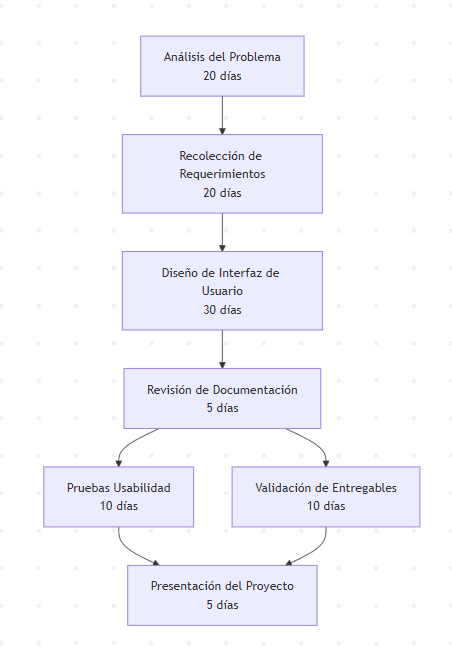
\includegraphics[width=0.60\textwidth,keepaspectratio]{./Media/Ruta Critica V3.png}%
  }
  \caption{Mapa visual de la Ruta Crítica del proyecto}
\end{figure}


\clearpage
\section{Estimación Costo Inicial}
\subsection{Tabla de Costos Estimados}
\begin{table}[h!]
    \centering
    \begin{tabular}{lrrr}
        \toprule
        \textbf{Concepto} & \textbf{Tarifa/Hora (MX)} & \textbf{Horas Estimadas} & \textbf{Total (MX)} \\
        \midrule
        Líder de Proyecto Jr & 156.25 & 800 & 124,800 \\
        Analista Jr & 125 & 800 & 100,000 \\
        Diseñador UI/UX Jr & 125 & 480 & 30,000 \\
        QA Jr & 113 & 240 & 54,240 \\
        Desarrollador Mobile Jr & 225 & 480 & 108,000 \\
        Cámaras de reconocimiento facial (3) &  &  & 7,500 \\
        Servidores en la nube &  &  & 6,250 \\
        Licencias de software &  &  & 3,000 \\
        Internet y servicios de red &  &  & 2,500 \\
        Material de oficina y papelería &  &  & 1,250 \\
        \midrule
    	\textbf{Subtotal}      &     &     & 442,540 \\
    	\textbf{Contingencia (20\%)} & &  & 88,508 \\
    \midrule
    	\textbf{Total Estimado} &     &     & \textbf{531,048} \\
        \bottomrule
    \end{tabular}
    \caption{Estimación de costos reales y desglosados para el proyecto Argos.}
\end{table}
\subsection{Fórmula de Contingencia}
La contingencia se calcula como:
\[
\text{Costo Final} = \text{Subtotal} + (\text{Subtotal} \times \text{Porcentaje de Contingencia})
\]

\clearpage
\section{Análisis de Costos y Esfuerzo (Método COCOMO)}

Para estimar el esfuerzo y el tiempo del proyecto \textit{Argos}, hemos utilizado el modelo COCOMO (Modelo Constructivo de Costos) en su versión intermedia. Este método se basa en el tamaño del software y en una serie de factores de costo para generar una estimación realista.

\subsection{Estimación del Tamaño del Software (KLOC)}
Debido a que el proyecto se encuentra en una etapa de planeación, el tamaño del software se ha estimado en *25,000 líneas de código (25 KLOC)*. Esta cifra se considera apropiada para una solución integral que incluye un sistema de reconocimiento facial, una aplicación móvil, una página web y la infraestructura de base de datos para el almacenamiento seguro de la información.

\subsection{Cálculo del Esfuerzo y Tiempo del Proyecto}
El modelo COCOMO intermedio se basa en dos ecuaciones principales:
\begin{itemize}
    \item *Esfuerzo (E):* Se mide en persona-mes.
    $E = a \times (\mathrm{KLOC})^{b} \times \mathrm{EAF}$
    \item *Tiempo de Desarrollo (TDEV):* Se mide en meses.
    $TDEV = c \times (\mathrm{E})^{d}$
\end{itemize}
Para un proyecto de tipo \textbf{semi-independiente} (considerando la naturaleza del proyecto que combina elementos de innovación con requisitos bien definidos), los coeficientes son: $a=3.0$, $b=1.12$, $c=2.5$ y $d=0.35$.

\subsubsection{Factores de Costo (EAF - \textit{Effort Adjustment Factor})}
Hemos asignado valores a los factores de costo (EAF) con base en la información del proyecto y sus características.

\begin{enumerate}
    \item \textbf{Atributos del Producto}
    \begin{itemize}
        \item Fiabilidad requerida del software (\textit{RELY}): 1.15 (Alta)
        \item Tamaño de la base de datos (\textit{DATA}): 1.00 (Nominal)
        \item Complejidad del producto (\textit{CPLX}): 1.29 (Muy Alta)
    \end{itemize}
    \item \textbf{Atributos del Hardware}
    \begin{itemize}
        \item Restricciones de tiempo de ejecución (\textit{TIME}): 1.00 (Nominal)
        \item Restricciones de memoria principal (\textit{STOR}): 1.00 (Nominal)
        \item Volatilidad del entorno de la máquina virtual (\textit{VIRT}): 0.94 (Baja)
        \item Tiempo de respuesta del sistema (\textit{TURN}): 1.07 (Alta)
    \end{itemize}
    \item \textbf{Atributos del Personal}
    \begin{itemize}
        \item Capacidad del analista (\textit{ACAP}): 1.00 (Nominal)
        \item Experiencia en la aplicación (\textit{AEXP}): 1.00 (Nominal)
        \item Capacidad del programador (\textit{PCAP}): 1.00 (Nominal)
        \item Experiencia en la máquina virtual (\textit{VEXP}): 1.00 (Nominal)
        \item Experiencia en el lenguaje de programación (\textit{LEXP}): 1.00 (Nominal)
    \end{itemize}
    \item \textbf{Atributos del Proyecto}
    \begin{itemize}
        \item Uso de herramientas de software (\textit{TOOL}): 1.00 (Nominal)
        \item Cumplimiento de plazos del proyecto (\textit{SCED}): 1.11 (Alta)
    \end{itemize}
\end{enumerate}

El \textbf{EAF} se calcula multiplicando todos estos factores de costo:
$EAF = 1.15 \times 1.00 \times 1.29 \times 1.00 \times 1.00 \times 0.94 \times 1.07 \times 1.00 \times 1.00 \times 1.00 \times 1.00 \times 1.00 \times 1.00 \times 1.11 \approx 1.83$
 3. Resultados del Cálculo
Aplicando las fórmulas con los valores estimados, obtenemos:
\begin{itemize}
    \item \textbf{Cálculo del Esfuerzo (E):}
    $E = 3.0 \times \left(25\right)^{1.12} \times 1.83 \approx 199.1$ persona-mes.
    \item \textbf{Cálculo del Tiempo de Desarrollo (TDEV):}
    $TDEV = 2.5 \times \left(199.1\right)^{0.35} \approx 18.2$ meses.
\end{itemize}

4. Conclusiones
Los resultados del modelo COCOMO intermedio indican que el proyecto \textit{Argos} requerirá:
\begin{itemize}
    \item Un \textbf{esfuerzo total} de aproximadamente \textbf{199.1 persona-mes}.
    \item Un \textbf{tiempo de desarrollo} de \textbf{18.2 meses}.
    \item Un \textbf{equipo promedio} de $\frac{199.1\ \mathrm{persona-mes}}{18.2\ \mathrm{meses}} \approx 11$ personas.
\end{itemize}
Esta estimación valida la complejidad y el alcance del proyecto, demostrando que para su correcta ejecución se necesita un equipo de desarrollo más grande y un cronograma más extenso que el planteado en el Diagrama de Gantt inicial. La duración de 105 días hábiles (aproximadamente 5 meses) mencionada en la planeación se enfoca en las primeras etapas de análisis y diseño, no en la implementación completa del sistema.
%%==========================================================================================%

\clearpage
\chapter{Requerimientos y Normativas}


\section{Requerimientos Funcionales}

\begin{table}[htbp]
    \centering
    \caption{Tabla de requerimientos funcionales}
    \label{tab:requerimientos_funcionales}
    \normalsize
    \renewcommand{\arraystretch}{1.7}
    \setlength{\tabcolsep}{12pt}
    \rowcolors{2}{gray!10}{white}
    \begin{tabularx}{\linewidth}{>{\columncolor{gray!20}}m{1.5cm} >{\columncolor{white}}m{3.2cm} >{\raggedright\arraybackslash\columncolor{white}}X >{\columncolor{gray!10}}m{2.2cm}}
    \toprule
    \rowcolor{gray!40}
    \textcolor{black}{\textbf{ID}} & \textcolor{black}{\textbf{Requerimiento}} & \textcolor{black}{\textbf{Descripción}} & \textcolor{black}{\textbf{Prioridad}} \\
    \midrule
    RF-001 & Registro facial & Implementar mecanismo de reconocimiento facial para registro automático de entrada del alumnado. & \textbf{Alta} \\
    RF-002 & Herramienta docente & Proporcionar herramienta digital a docentes para verificar/registrar asistencia. & \textbf{Media} \\
    RF-003 & Consulta padres & Plataforma en línea para consulta de asistencia en tiempo real por padres. & \textbf{Media} \\
    RF-004 & Control de acceso & Restricción de acceso a personas no autorizadas con validaciones técnicas. & \textbf{Alta} \\
    RF-005 & Gestión de datos & Gestión segura de información de accesos y asistencia escolar. & \textbf{Alta} \\
    \bottomrule
    \end{tabularx}
\end{table}

\clearpage
\section{Necesidades de Usuario}

Se realizó una encuesta a estudiantes y docentes de la UPP para conocer su percepción sobre el sistema de control de acceso y la posible implementación de reconocimiento facial. Los resultados clave fueron:

\begin{itemize}
    \item El 97.6\% desea un acceso más seguro.
    \item Las opciones preferidas para un nuevo sistema son: credenciales magnéticas (51.2\%), huella digital (41.5\%) y reconocimiento facial (36.6\%).
    \item El 90.2\% estaría dispuesto a proporcionar su imagen para el acceso.
    \item Las principales preocupaciones son la seguridad de la información (53.7\%), errores del sistema (39\%), privacidad de datos (36.6\%) y la incomodidad por grabación (19.5\%).
    \item Necesidades principales: reducción de tiempos de espera (85\%), facilidad de uso (90\%), consulta en tiempo real (72\%) y seguridad y privacidad de datos (68\%).
\end{itemize}

En conclusión, existe una demanda clara por un sistema de acceso más eficiente y seguro. El reconocimiento facial es viable si se prioriza la protección de datos y se informa adecuadamente a los usuarios.

\begin{table}[H]
\centering
\caption{Resumen de Respuestas de la Encuesta}
\begin{tabular}{|p{6cm}|c|}
\hline
\rowcolor[HTML]{CFE2F3}\textbf{Necesidad Identificada} & \textbf{Porcentaje (\%)} \\
\hline
Reducción de tiempos de espera & 85 \\
Facilidad de uso & 90 \\
Consulta en tiempo real & 72 \\
Seguridad y privacidad de datos & 68 \\
\hline
\end{tabular}
\end{table}

\begin{figure}[H]
\centering
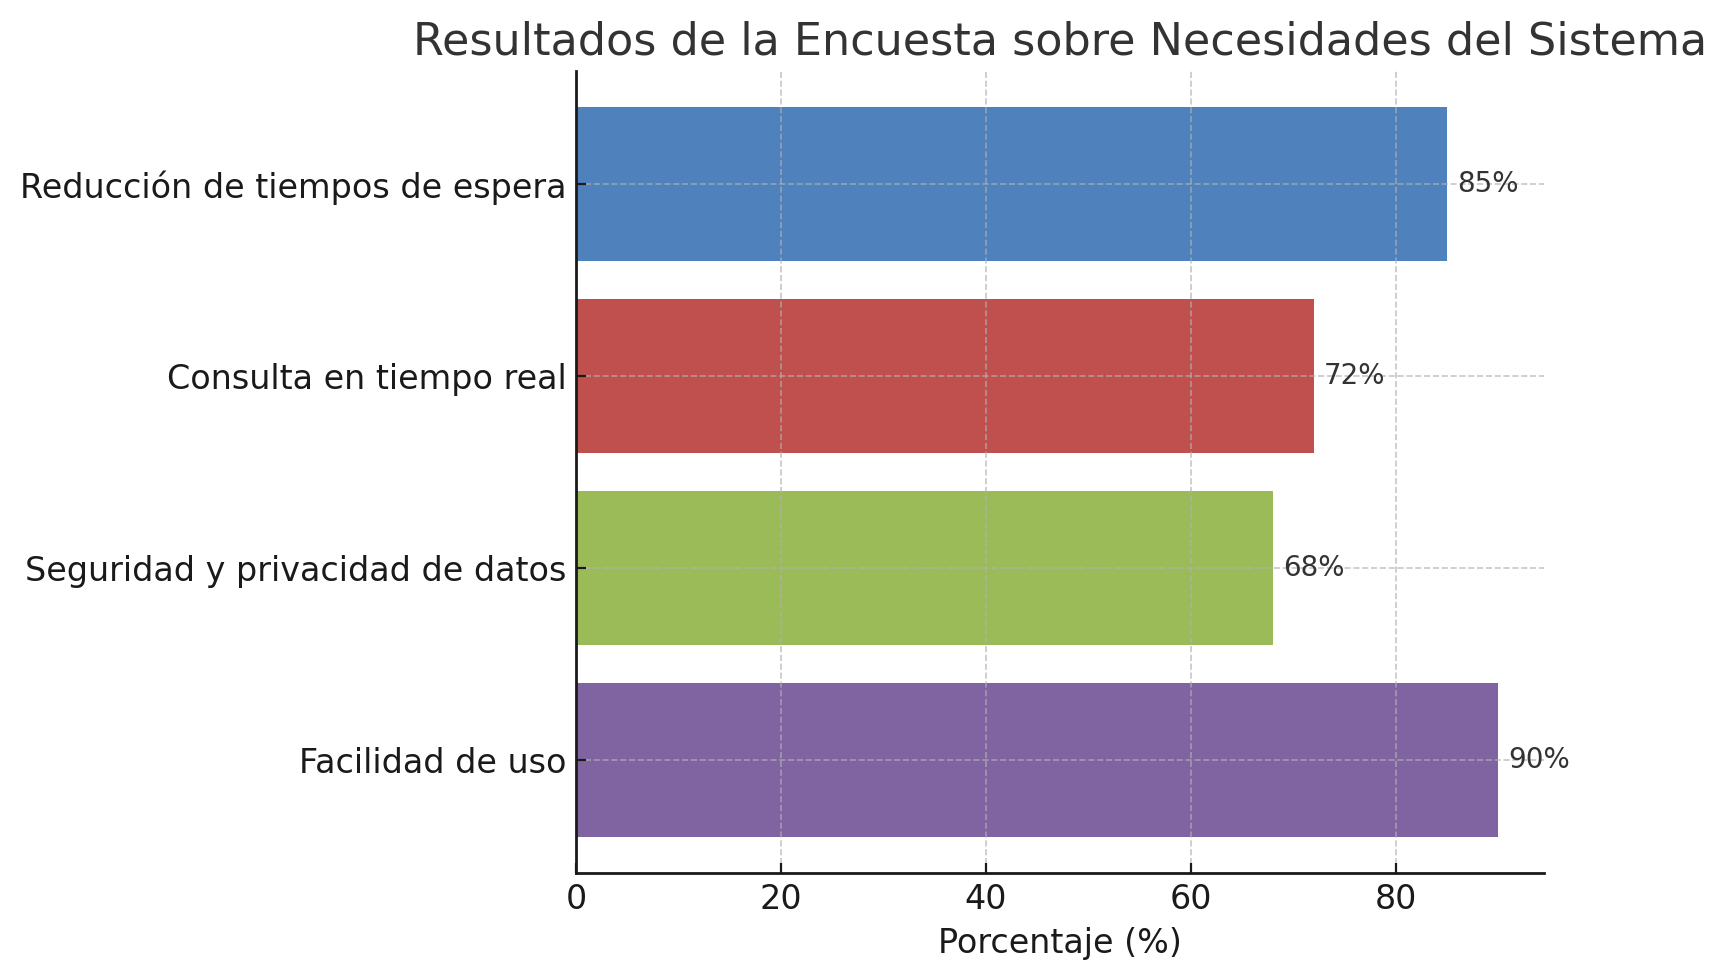
\includegraphics[width=0.8\textwidth]{./Media/grafico_encuesta.png}
\caption{Resultados de la encuesta sobre necesidades del sistema}
\end{figure}

\clearpage
\section{Normativas}

Para asegurar la calidad y seguridad en el Proyecto Argos, se adoptaron las siguientes normativas internacionales clave. Estas guían el desarrollo, la gestión y la protección de la información en el sistema:

\subsubsection*{ISO 9001:2015 – Sistemas de Gestión de la Calidad}
Establece un sistema de gestión de calidad basado en la mejora continua y la satisfacción del cliente. En Argos, se aplica para documentar procesos, auditar actividades clave y asegurar que cada entregable cumpla los requisitos funcionales y no funcionales definidos desde el inicio del proyecto.

\subsubsection*{ISO/IEC 25000 – Calidad del Producto de Software (SQuaRE)}
Proporciona criterios para evaluar la calidad del software en funcionalidad, usabilidad y eficiencia. Permite definir atributos medibles, estandarizar pruebas con usuarios finales (alumnos, docentes y padres de familia) y detectar posibles mejoras antes de la implementación final.

\subsubsection*{ISO/IEC 27001 – Seguridad de la Información}
Se enfoca en la gestión de la seguridad de la información, esencial para proteger los datos biométricos y registros de asistencia. Incluye prácticas de gestión de riesgos, uso de cifrado y autenticación segura, así como políticas de respaldo y recuperación ante incidentes.

\subsubsection*{ISO/IEC 29110 – Ingeniería de Software para PYMES y Equipos Pequeños}
Pensada para proyectos pequeños, facilita la documentación simple, la definición clara de roles y responsabilidades, y la adopción de procesos ágiles y estructurados en las fases de diseño, codificación, pruebas y validación del sistema.

\subsubsection*{Conclusión}
La integración de estas normativas fortalece la calidad y seguridad del sistema, asegurando un producto confiable, seguro y alineado con estándares internacionales. El Encargado de Calidad supervisa su aplicación y verifica, mediante auditorías internas, que cada práctica esté alineada con estos lineamientos.


%%==========================================================================================%

\clearpage
\chapter{Diseño de la UI}


\section{Logo Empresarial}

El logo de \textbf{SafeSight} representa la identidad y misión del equipo. Su diseño es moderno y claro, y comunica seguridad y tecnología de visión.

\begin{figure}[h!]
		\centering
		% Se muestra la imagen si existe; en caso contrario, se deja un marcador visual.
		\IfFileExists{./Media/Empresa.jpg}{%
			
\includegraphics[width=0.3\textwidth]{./Media/Empresa.jpg}%
		}{%
			\fbox{\parbox{0.3\textwidth}{\centering Imagen ``Empresa.jpg'' no disponible}}%
		}
		\caption{Logotipo oficial del equipo desarrollador SafeSight.}\label{fig:logo_safesight}
\end{figure}

\subsection*{Justificación del Diseño}

El diseño fusiona seguridad y monitoreo avanzado.

\begin{itemize}
\item \textbf{Ojo central:} Representa visión, inteligencia y precisión.
\item \textbf{Red de nodos:} Simboliza protección integral de usuarios y datos.
\item \textbf{Círculo exterior:} Refuerza seguridad y control total.
\end{itemize}

	extit{Visión segura}: tecnología que vigila y protege el entorno.

\subsection*{Paleta de Colores}

Colores que transmiten profesionalismo y seguridad tecnológica.

\begin{itemize}
\item \textbf{Azul:} Confianza y estabilidad.
\item \textbf{Verde azulado:} Innovación y claridad.
\item \textbf{Verde claro:} Seguridad y positividad.
\end{itemize}

\subsection*{Tipografía}

Tipografía \textbf{sans-serif} moderna y geométrica, con CamelCase para destacar la unión de ``Safe'' y ``Sight''.



\clearpage

\section{Logo Aplicación}

El logotipo de la aplicación \textbf{Argos} identifica el sistema ante los usuarios. Es minimalista y tecnológico; comunica precisión, enfoque e identificación.

\begin{figure}[h!]
		\centering
		% Se muestra la imagen si existe
		\IfFileExists{./Media/Argos 2.png}{%
			
\includegraphics[width=0.3\textwidth]{./Media/Argos 2.png}%
		}{%
			\fbox{\parbox{0.3\textwidth}{\centering Imagen ``Argos 2.jpg'' no disponible}}%
		}
		\caption{Logotipo oficial de la aplicación Argos.}\label{fig:logo_argos}
\end{figure}

\subsection*{Justificación del Diseño}

El concepto refleja la función principal: reconocimiento mediante un marco digital.

\begin{itemize}
		\item \textbf{Elemento central:} Letra “A” mayúscula estilizada que representa “Argos”. Geométrica y limpia; moderna y estable.
		\item \textbf{Marco de enfoque:} La “A” se enmarca con dos corchetes superiores (\texttt{[ ]}) que evocan el marco de una cámara. Comunica escanear, enfocar e identificar.
		\item \textbf{Mensaje general:} Imagen de alta tecnología y precisión; “Argos” como herramienta de identificación.
\end{itemize}

\subsection*{Paleta de Colores}

Paleta monocromática de alto contraste (blanco y negro):

\begin{itemize}
		\item \textbf{Claridad y legibilidad:} Reconocimiento inmediato en cualquier fondo.
		\item \textbf{Modernidad y seriedad:} Estética funcional propia de aplicaciones tecnológicas.
		\item \textbf{Versatilidad:} Se integra con paletas institucionales sin perder identidad.
\end{itemize}

\subsection*{Tipografía}

“ARGOS” usa tipografía \textbf{sans-serif geométrica y en mayúsculas}. Robusta y clara; transmite fiabilidad y solidez.

\subsection*{Aplicación como Icono}

El isotipo (la “A” enmarcada) funciona muy bien como icono en móviles y mantiene legibilidad en tamaños pequeños.


\clearpage
\section{Wireframes}

\subsection{ Pantalla Principal de Selección de Rol}
\begin{samepage}\small
Esta es la primera pantalla que encuentra el usuario al abrir la aplicación, funcionando como un portal de bienvenida y un punto de navegación inicial. Su propósito es segmentar a los usuarios desde el principio, permitiendo que cada tipo de usuario acceda a su respectivo flujo de inicio de sesión de manera clara y directa. Este diseño evita una interfaz de login genérica y confusa, que requeriría que el usuario especifique su rol mediante un menú desplegable, simplificando así el primer paso de interacción con la aplicación.
\begin{figure}[H]
    \centering
    \IfFileExists{./Media/Wireframes/Page Main.png}{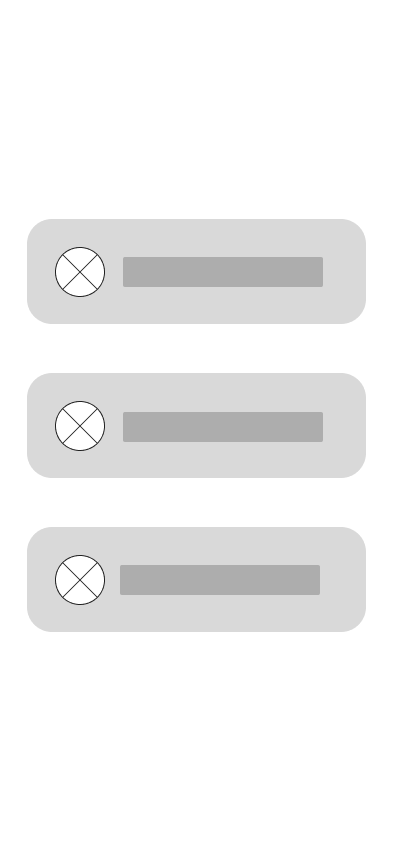
\includegraphics[width=0.28\textwidth]{./Media/Wireframes/Page Main.png}}{\fbox{\parbox{0.28\textwidth}{\centering Imagen ``Page Main.png'' no disponible}}}
    \caption{Wireframe de la pantalla de selección de rol.}\label{fig:wf-main}
\end{figure}
    \subsubsection*{Análisis de Componentes y Diseño}
    El diseño se basa en la simplicidad y la claridad. La pantalla presenta tres botones de selección de gran tamaño, dispuestos verticalmente, optimizados para una fácil interacción en dispositivos móviles donde el espacio táctil es primordial. Cada botón está diseñado para representar un rol principal (Estudiante, Docente y Padre de Familia) y reserva un espacio para un icono representativo que ayuda en la identificación visual rápida, junto con un área para el texto descriptivo del rol. La ausencia de otros elementos en la pantalla centra toda la atención del usuario en una única decisión: identificar su perfil.
    
    \subsubsection*{Flujo de Usuario y Funcionalidad}
    El flujo es directo y sin fricciones. El usuario identifica visualmente su rol, pulsa la opción correspondiente y la aplicación lo redirige a la pantalla de inicio de sesión específica para ese perfil. Este paso previo es crucial para personalizar la experiencia del usuario desde el primer momento. Al segmentar los flujos, la aplicación puede presentar a cada usuario únicamente la información y las herramientas que son relevantes para él, simplificando las interfaces subsecuentes y reduciendo la carga cognitiva.
\normalsize\end{samepage}
\clearpage

\subsection{ Pantalla de Inicio de Sesión (Estudiante)}
\begin{samepage}\small
Tras seleccionar el rol ``Estudiante'', el usuario es dirigido a esta interfaz de autenticación. Su diseño es limpio y centrado en la tarea, eliminando cualquier distracción para facilitar un acceso rápido y seguro a la plataforma. El uso del correo institucional como método de identificación estandariza el acceso para todo el alumnado, utilizando una credencial que ya les es familiar y que forma parte de su identidad digital dentro de la universidad.
\begin{figure}[H]\centering
    \IfFileExists{./Media/Wireframes/Login Student.png}{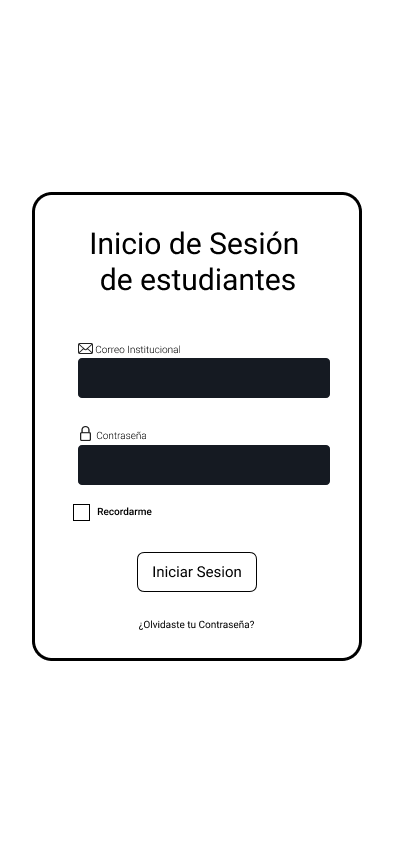
\includegraphics[width=0.28\textwidth]{./Media/Wireframes/Login Student.png}}{\fbox{\parbox{0.28\textwidth}{\centering Imagen ``Login Student.png'' no disponible}}}
    \caption{Wireframe de la pantalla de inicio de sesión para estudiantes.}\label{fig:wf-login-student}
\end{figure}
    \subsubsection*{Análisis de Componentes y Diseño}
    La jerarquía visual de la pantalla guía al usuario de forma natural. Incluye un título claro (``Inicio de Sesión de estudiantes''), seguido de dos campos de entrada bien definidos para ``Correo Institucional'' y ``Contraseña''. El checkbox para ``Recordarme'' es una función de conveniencia que reduce la fricción en usos futuros. El botón de acción principal (CTA) ``Iniciar Sesion'' está prominentemente ubicado, y un enlace discreto para recuperar la contraseña ofrece una solución a un problema común sin desviar la atención de la tarea principal.
    
    \subsubsection*{Flujo de Usuario y Funcionalidad}
    El usuario introduce sus credenciales para ser validado por el sistema. Esta pantalla actúa como una puerta de seguridad para proteger la información personal del alumno. Si la autenticación es correcta, el sistema le da acceso directo a su Panel del Alumno, su centro de información personal. En caso de error, se mostraría un mensaje informativo y no intrusivo para guiarlo en la corrección de los datos, evitando la frustración.
\normalsize\end{samepage}
\clearpage

\subsection{ Panel del Alumno}
\begin{samepage}\small
Esta pantalla es el centro de información principal para el estudiante; una herramienta de autogestión que le permite estar al tanto de su rendimiento y fomenta la responsabilidad sobre su asistencia. El diseño busca empoderar al estudiante, dándole acceso transparente, inmediato y comprensible a sus datos de asistencia, lo cual es un objetivo clave del proyecto Argos.
\begin{figure}[H]\centering
    \IfFileExists{./Media/Wireframes/Page Student.png}{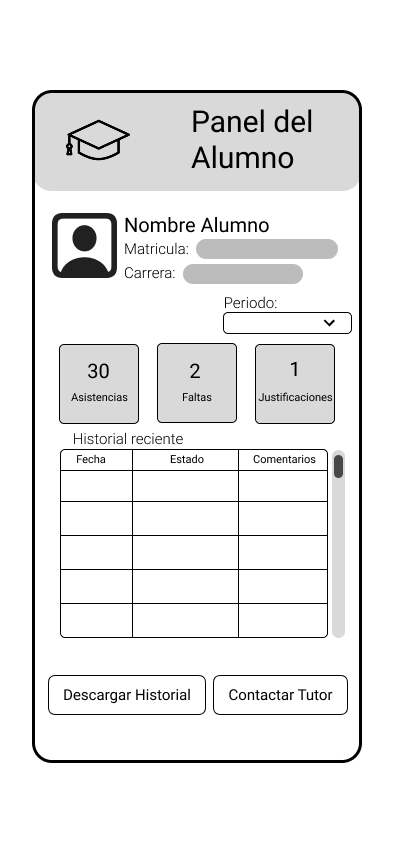
\includegraphics[width=0.28\textwidth]{./Media/Wireframes/Page Student.png}}{\fbox{\parbox{0.28\textwidth}{\centering Imagen ``Page Student.png'' no disponible}}}
    \caption{Wireframe del panel principal del alumno.}\label{fig:wf-student-panel}
\end{figure}
    \subsubsection*{Análisis de Componentes y Diseño}
    La interfaz presenta un encabezado con los datos del alumno (foto, nombre, matrícula), un selector para filtrar por periodo académico, tres tarjetas de resumen que ofrecen una vista cuantitativa inmediata de ``Asistencias'', ``Faltas'' y ``Justificaciones'', una tabla con el historial reciente para una revisión detallada, y botones de acción para ``Descargar Historial'' y ``Contactar Tutor''. El diseño prioriza la información más importante en la parte superior, permitiendo una lectura rápida y eficiente.
    
    \subsubsection*{Flujo de Usuario y Funcionalidad}
    Esta pantalla permite al estudiante verificar su estado de un solo vistazo, filtrar su historial por distintos periodos académicos, generar reportes oficiales en formato PDF para posibles trámites administrativos, e iniciar comunicación directa con su tutor para resolver dudas o aclarar inconsistencias. No es solo un repositorio de datos, sino una herramienta interactiva que promueve la autogestión.
\normalsize\end{samepage}
\clearpage

\subsection{ Pantalla de Inicio de Sesión (Docente)}
\begin{samepage}\small
Interfaz de autenticación diseñada específicamente para el personal docente de la institución. El uso de la matrícula como identificador asegura un método de acceso estandarizado y formal, alineado con los sistemas de gestión internos y diferenciando claramente el acceso del personal del de los alumnos. La consistencia visual con las otras pantallas de login reduce la curva de aprendizaje.
\begin{figure}[H]\centering
    \IfFileExists{./Media/Wireframes/Login Teacher.png}{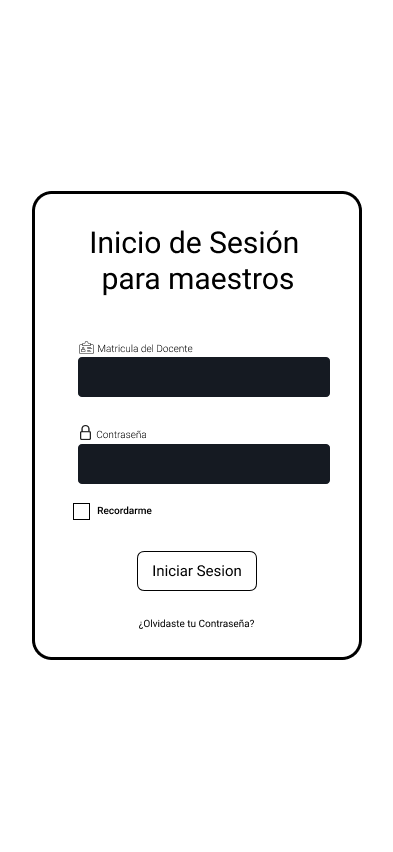
\includegraphics[width=0.28\textwidth]{./Media/Wireframes/Login Teacher.png}}{\fbox{\parbox{0.28\textwidth}{\centering Imagen ``Login Teacher.png'' no disponible}}}
    \caption{Wireframe de la pantalla de inicio de sesión para docentes.}\label{fig:wf-login-teacher}
\end{figure}
    \subsubsection*{Análisis de Componentes y Diseño}
    La pantalla contiene un título, un campo específico para la ``Matrícula del Docente'' como identificador único, un campo de contraseña y las opciones comunes que mantienen la consistencia en la experiencia de usuario a través de toda la aplicación (Recordarme, Iniciar sesión, ¿Olvidaste tu contraseña?). El diseño es deliberadamente simple para enfocarse en una única acción: la autenticación segura.
    
    \subsubsection*{Flujo de Usuario y Funcionalidad}
    El docente introduce su matrícula y contraseña para ser autenticado. Una vez validado, el sistema le concede acceso a sus herramientas de gestión de asistencia, como el panel de pase de lista. Este paso de validación es una medida de seguridad crítica para asegurar que la información sensible de los alumnos solo sea accesible y modificable por personal autorizado.
\normalsize\end{samepage}
\clearpage

\subsection{ Panel del Docente (Pase de Lista)}
\begin{samepage}\small
Esta es la herramienta principal y de uso diario para los maestros. Su diseño está optimizado para que el proceso de registrar la asistencia en el aula sea una tarea rápida, eficiente y con una mínima carga cognitiva, permitiendo al docente enfocarse en sus alumnos en lugar de en la herramienta administrativa. El objetivo es que el pase de lista tome solo un par de minutos al inicio de la clase.
\begin{figure}[H]\centering
    \IfFileExists{./Media/Wireframes/Page Teacher.png}{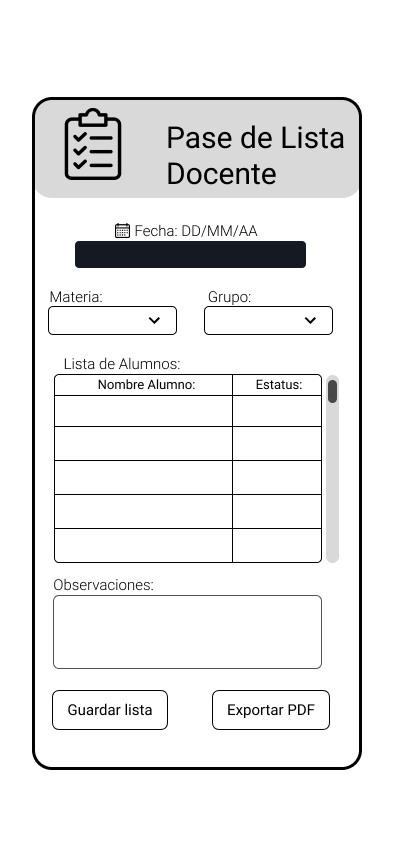
\includegraphics[width=0.28\textwidth]{./Media/Wireframes/Page Teacher.png}}{\fbox{\parbox{0.28\textwidth}{\centering Imagen ``Page Teacher.png'' no disponible}}}
    \caption{Wireframe del panel de pase de lista del docente.}\label{fig:wf-teacher-panel}
\end{figure}
    \subsubsection*{Análisis de Componentes y Diseño}
    La interfaz incluye selectores desplegables para ``Materia'' y ``Grupo'' que actúan como filtros para cargar la lista de alumnos correcta, un campo de ``Fecha'', la lista de alumnos con su estatus, un área de texto para ``Observaciones'' y los botones de acción ``Guardar lista'' y ``Exportar PDF''. La disposición vertical de los elementos guía al docente a través del proceso de forma lógica, de arriba hacia abajo.
    
    \subsubsection*{Flujo de Usuario y Funcionalidad}
    El flujo de trabajo es lineal e intuitivo: el docente selecciona la clase y grupo, la aplicación carga la lista de estudiantes correspondiente, el docente registra el estatus de cada alumno, añade notas generales si es necesario (ej. ``Actividad de laboratorio''), y finalmente guarda el registro del día en la base de datos o lo exporta para sus archivos personales.
\normalsize\end{samepage}
\clearpage

\subsection{ Pantalla de Inicio de Sesión (Padres de Familia)}
\begin{samepage}\small
Pantalla de acceso para los padres o tutores, diseñada para permitirles el monitoreo del estudiante de una forma segura y controlada. El uso de la matrícula del alumno como una referencia directa es una decisión de diseño clave para asegurar que el padre se vincule inequívocamente con la información de su hijo, garantizando la privacidad y la correcta asignación de datos.
\begin{figure}[H]\centering
    \IfFileExists{./Media/Wireframes/Login Parents.png}{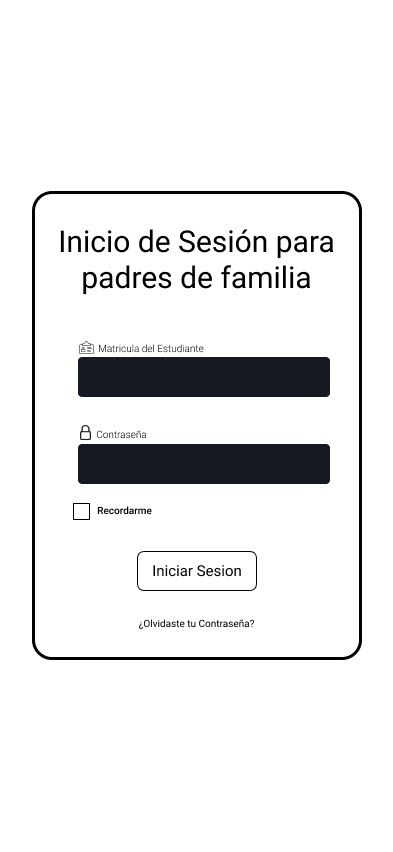
\includegraphics[width=0.28\textwidth]{./Media/Wireframes/Login Parents.png}}{\fbox{\parbox{0.28\textwidth}{\centering Imagen ``Login Parents.png'' no disponible}}}
    \caption{Wireframe de la pantalla de inicio de sesión para padres.}\label{fig:wf-login-parents}
\end{figure}
    \subsubsection*{Análisis de Componentes y Diseño}
    La interfaz incluye el título, un campo clave para la ``Matrícula del Estudiante'' que se va a consultar, el campo de contraseña y las opciones comunes de inicio de sesión. La simplicidad del diseño busca acomodar a usuarios con diferentes niveles de habilidad tecnológica, enfocándose únicamente en la información esencial para el acceso.
    
    \subsubsection*{Flujo de Usuario y Funcionalidad}
    El padre de familia se autentica utilizando la matrícula de su hijo o tutelado y su propia contraseña. Este método de doble factor (algo que el alumno tiene y algo que el padre sabe) asegura que solo tenga acceso a la información del estudiante correcto, respetando la privacidad de los datos, para después ingresar al panel de seguimiento.
\normalsize\end{samepage}
\clearpage

\subsection{ Panel de Padres de Familia}
\begin{samepage}\small
Interfaz diseñada para que los padres puedan consultar y visualizar de manera sencilla el historial de asistencia de sus hijos. Actúa como un puente de comunicación y seguimiento entre el hogar y la institución, fomentando una colaboración proactiva en la educación del alumno y aumentando la transparencia, uno de los objetivos del proyecto.
\begin{figure}[H]\centering
    \IfFileExists{./Media/Wireframes/Page Parents.png}{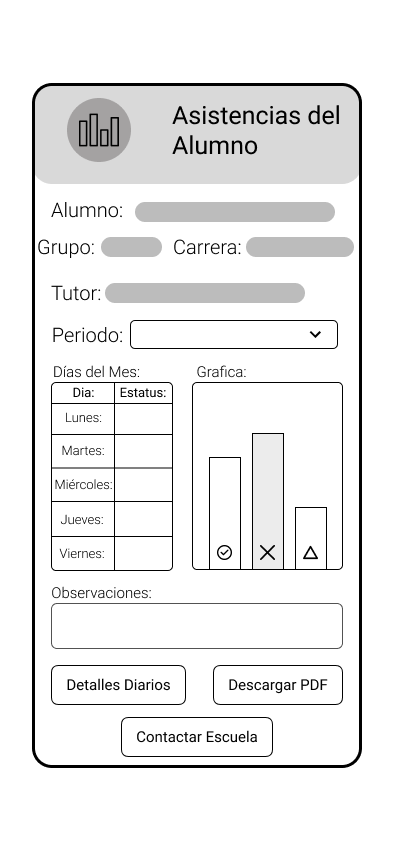
\includegraphics[width=0.28\textwidth]{./Media/Wireframes/Page Parents.png}}{\fbox{\parbox{0.28\textwidth}{\centering Imagen ``Page Parents.png'' no disponible}}}
    \caption{Wireframe del panel de seguimiento para padres.}\label{fig:wf-parents-panel}
\end{figure}
    \subsubsection*{Análisis de Componentes y Diseño}
    La pantalla muestra la información del alumno, una tabla de estatus por día para revisión detallada, y una gráfica de barras para un resumen visual rápido que facilita la identificación de patrones o tendencias (ej. ausencias recurrentes en un día específico). Los botones de acción ``Detalles Diarios'', ``Descargar PDF'' y ``Contactar Escuela'' están claramente visibles para promover la acción.
    
    \subsubsection*{Flujo de Usuario y Funcionalidad}
    Permite a los padres revisar el historial de asistencia, visualizar tendencias a través de gráficos para una fácil interpretación, descargar reportes y contactar a la institución directamente desde la aplicación. Este flujo completo, desde la visualización de datos hasta la comunicación, cierra el ciclo de monitoreo y acción.
\normalsize\end{samepage}

\clearpage
\subsection{ Pantalla de Carga}
\begin{samepage}\small
Pantalla intermedia que mejora la experiencia de usuario al proporcionar retroalimentación visual durante los tiempos de espera del sistema. Su función es gestionar la percepción del tiempo, reduciendo la incertidumbre y la sensación de lentitud de la aplicación mientras se procesan datos en segundo plano.
\begin{figure}[H]\centering
    \IfFileExists{./Media/Wireframes/Page Loader.png}{
\includegraphics[width=0.28\textwidth]{./Media/Wireframes/Page Loader.png}}{\fbox{\parbox{0.28\textwidth}{\centering Imagen ``Page Loader.png'' no disponible}}}
    \caption{Wireframe de la pantalla de carga.}\label{fig:wf-loader}
\end{figure}
    \subsubsection*{Análisis de Componentes y Diseño}
    El diseño es minimalista para no distraer. Consiste en un contenedor circular en la parte superior, ideal para mostrar el logo de Argos y reforzar la marca incluso en tiempos de espera, y un indicador de carga animado (spinner) en la parte inferior, un símbolo universal de que un proceso está en curso, lo que comunica claramente el estado del sistema al usuario.
    
    \subsubsection*{Flujo de Usuario y Funcionalidad}
    Esta pantalla aparece automáticamente en momentos clave, como después de iniciar sesión o al solicitar un reporte pesado, para informar al usuario que la aplicación está funcionando y procesando su solicitud. Este estado intermedio es crítico para prevenir la frustración y el posible abandono de la tarea por parte del usuario, haciendo que la aplicación se sienta más robusta y responsiva.
\normalsize\end{samepage}

\clearpage
\section{Mockups}

\subsection{ Pantalla Principal de Selección de Rol}
\begin{samepage}\small
Esta pantalla es la puerta de entrada al ecosistema de Argos. Su diseño en modo oscuro (dark mode) establece un tono moderno y profesional desde el primer contacto. La interfaz está diseñada para ser extremadamente simple, guiando a los tres tipos de usuario a su respectivo flujo de trabajo sin ninguna ambigüedad, lo cual es fundamental para una buena primera impresión.
\begin{figure}[H]
	\centering
	\IfFileExists{./Media/Mockups/Page Main.png}{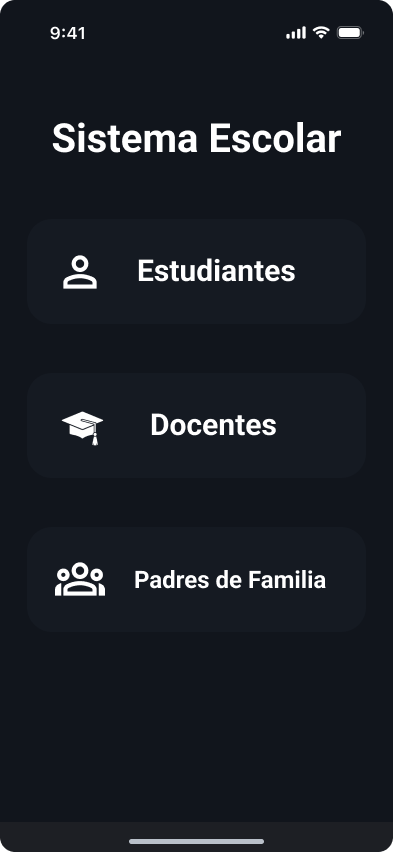
\includegraphics[width=0.28\textwidth]{./Media/Mockups/Page Main.png}}{\fbox{\parbox{0.28\textwidth}{\centering Imagen ``Page Main.png'' no disponible}}}
	\caption{Mockup de la pantalla de selección de rol.}\label{fig:mk-main}
\end{figure}
	\subsubsection*{Análisis de Diseño y Componentes}
	El diseño utiliza una paleta de colores basada en tonos de gris oscuro y carbón, con texto blanco de alto contraste para una legibilidad óptima. Los tres botones de selección para ``Estudiantes'', ``Docentes'' y ``Padres de Familia'' son los únicos elementos interactivos, ocupando un lugar central en la jerarquía visual. Su gran tamaño y esquinas redondeadas los hacen fácilmente pulsables en dispositivos táctiles. La inclusión de iconografía clara y universal (una persona, un birrete, un grupo de personas) junto al texto acelera el reconocimiento del rol.
    
	\subsubsection*{Flujo de Usuario y Funcionalidad}
	El flujo de usuario es intencionadamente lineal: el usuario abre la aplicación, se le presenta esta pantalla, identifica su rol y pulsa el botón correspondiente. Esta acción desencadena una transición a la pantalla de inicio de sesión específica para el perfil seleccionado, creando una experiencia de usuario segmentada y personalizada desde el inicio.
\normalsize\end{samepage}
\clearpage


\subsection{ Pantallas de Inicio de Sesión}
\begin{samepage}\small
Las tres pantallas de inicio de sesión (Estudiante, Docente y Padre de Familia) mantienen una consistencia de diseño casi total para reducir la carga cognitiva del usuario. La única variación significativa es el campo de identificación solicitado, lo cual personaliza el acceso para cada rol. El diseño limpio y enfocado elimina cualquier distracción, centrando al usuario en la tarea de autenticación.
\begin{figure}[H]
	\centering
	\IfFileExists{./Media/Mockups/Login Student.png}{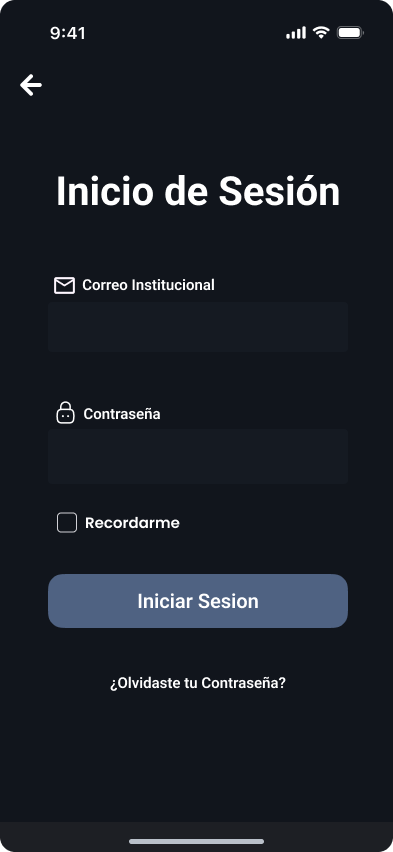
\includegraphics[width=0.22\textwidth]{./Media/Mockups/Login Student.png}}{\fbox{\parbox{0.22\textwidth}{\centering Login Student}}}
	\IfFileExists{./Media/Mockups/Login Teacher.png}{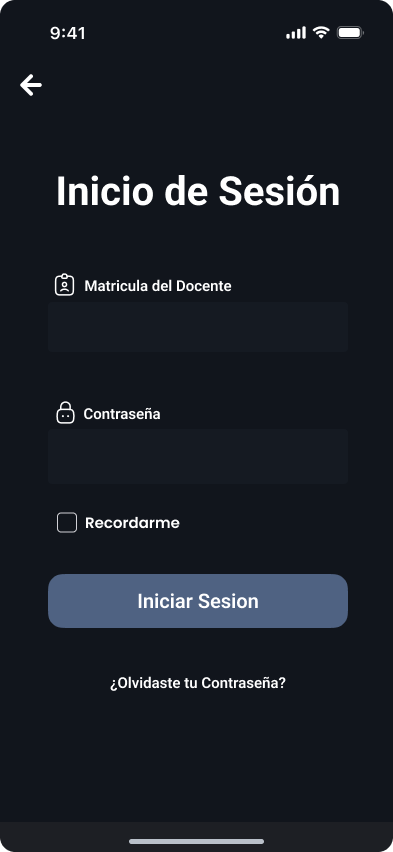
\includegraphics[width=0.22\textwidth]{./Media/Mockups/Login Teacher.png}}{\fbox{\parbox{0.22\textwidth}{\centering Login Teacher}}}
	\IfFileExists{./Media/Mockups/Login Parents.png}{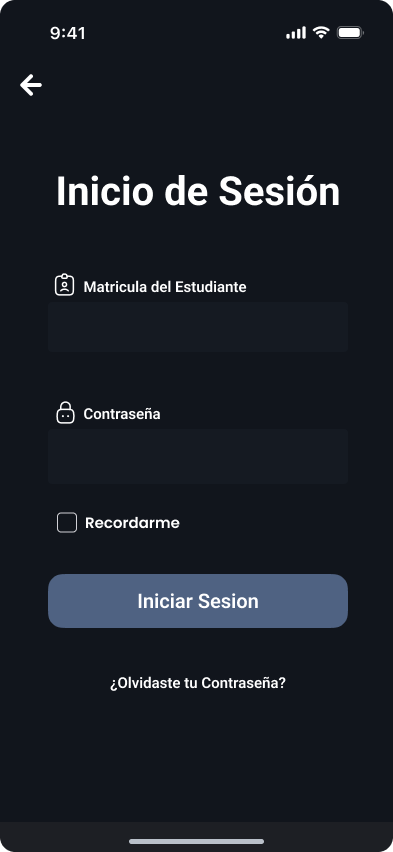
\includegraphics[width=0.22\textwidth]{./Media/Mockups/Login Parents.png}}{\fbox{\parbox{0.22\textwidth}{\centering Login Parents}}}
	\caption{Mockups de las pantallas de inicio de sesión para Estudiante, Docente y Padre de Familia.}\label{fig:mk-logins}
\end{figure}
	\subsubsection*{Análisis de Diseño y Componentes}
	Cada pantalla presenta un título claro, dos campos de entrada con íconos descriptivos, un checkbox para ``Recordarme'', un botón de acción principal (CTA) con un color de acento para destacar, y un enlace secundario para recuperar la contraseña. El campo de identificación cambia según el rol: ``Correo Institucional'' para estudiantes, ``Matrícula del Docente'' para maestros, y ``Matrícula del Estudiante'' para los padres, una decisión de diseño clave para alinear la aplicación con los sistemas de identificación de la institución.
    
	\subsubsection*{Flujo de Usuario y Funcionalidad}
	El usuario introduce sus credenciales y pulsa ``Iniciar Sesión''. El sistema valida la información contra la base de datos. Si la autenticación es exitosa, una pantalla de carga transitoria precede al acceso al panel principal correspondiente a su rol. En caso de error, se mostraría un mensaje específico para guiar al usuario.
\normalsize\end{samepage}
\clearpage

% --- Pantalla de Carga, Home Student, Attendance Student, Profile Student ---
\subsection{ Flujo del Estudiante}
\begin{samepage}\small
El flujo del estudiante está diseñado para ofrecerle una visión completa y clara de su estado académico en relación con la asistencia. La navegación se centra en un menú inferior persistente que le da acceso rápido a las secciones de Inicio, Asistencias y Perfil.
\begin{figure}[H]
	\centering
	\IfFileExists{./Media/Mockups/Home Student.png}{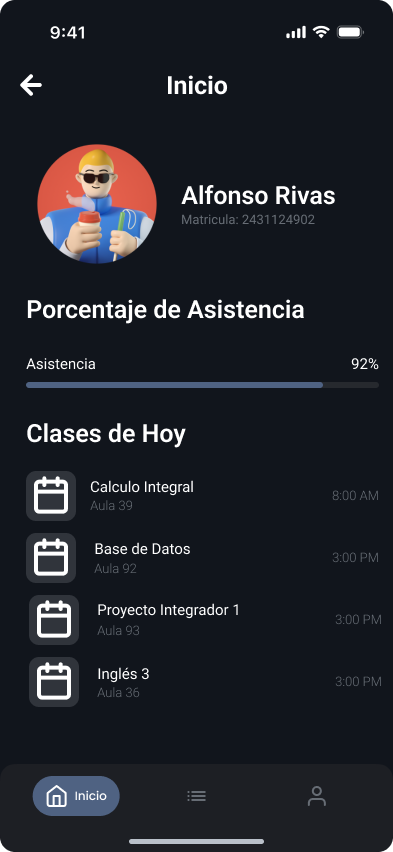
\includegraphics[width=0.22\textwidth]{./Media/Mockups/Home Student.png}}{\fbox{\parbox{0.22\textwidth}{\centering Home Student}}}
	\IfFileExists{./Media/Mockups/Attendance Student.png}{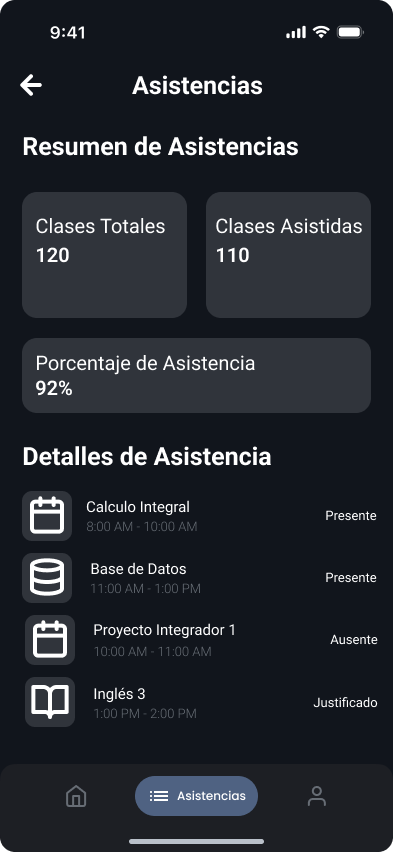
\includegraphics[width=0.22\textwidth]{./Media/Mockups/Attendance Student.png}}{\fbox{\parbox{0.22\textwidth}{\centering Attendance Student}}}
	\IfFileExists{./Media/Mockups/Profile Student.png}{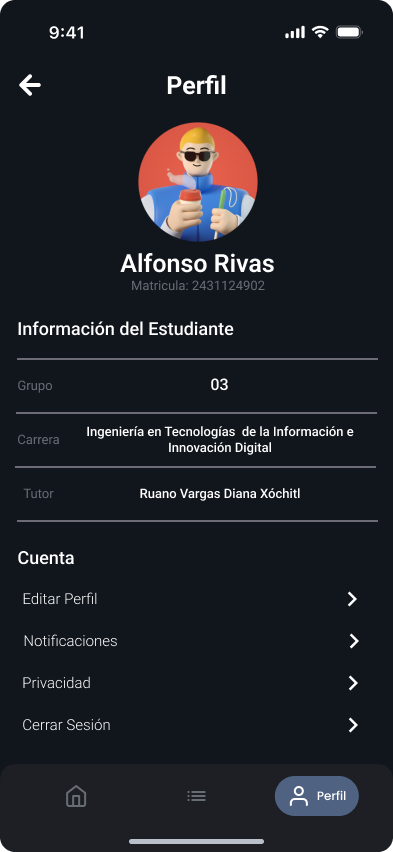
\includegraphics[width=0.22\textwidth]{./Media/Mockups/Profile Student.png}}{\fbox{\parbox{0.22\textwidth}{\centering Profile Student}}}
	\caption{Mockups del flujo del Estudiante: Inicio, Asistencias y Perfil.}\label{fig:mk-student-flow}
\end{figure}
	\subsubsection*{Análisis de Diseño y Componentes}
	La pantalla de \textbf{Inicio} (``Home Student.png'') actúa como un dashboard, personalizando la experiencia con un avatar 3D y mostrando la información más relevante del día: el porcentaje general de asistencia y la lista de clases programadas. La pantalla de \textbf{Asistencias} (``Attendance Student.png'') profundiza en los datos, usando tarjetas de resumen para métricas clave y una lista detallada que clasifica cada clase como ``Presente'', ``Ausente'' o ``Justificado''. La pantalla de \textbf{Perfil} (``Profile Student.png'') agrupa la información personal y las opciones de configuración de la cuenta (Editar Perfil, Notificaciones, etc.) de forma ordenada.
    
	\subsubsection*{Flujo de Usuario y Funcionalidad}
	Desde el inicio, el estudiante puede ver su agenda del día. Si desea más detalles, navega a la sección de Asistencias para un desglose completo. Finalmente, la sección de Perfil le permite gestionar su cuenta y cerrar la sesión de forma segura. El menú de navegación inferior garantiza que estas tres secciones clave estén siempre a un solo toque de distancia.
\normalsize\end{samepage}
\clearpage

% --- Flujo del Docente ---
\subsection{ Flujo del Docente}
\begin{samepage}\small
El flujo del docente está enfocado en la gestión y la eficiencia. Las herramientas están diseñadas para minimizar el tiempo administrativo y facilitar tanto el registro de la asistencia como la consulta de información general de sus grupos.
\begin{figure}[H]
	\centering
	\IfFileExists{./Media/Mockups/Chats.png}{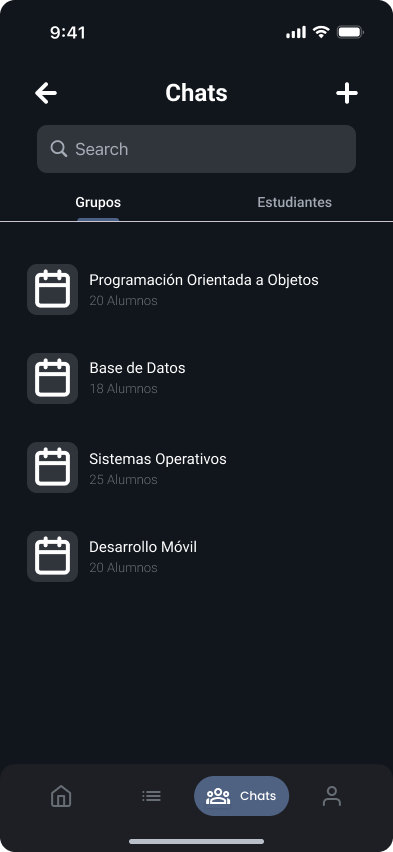
\includegraphics[width=0.22\textwidth]{./Media/Mockups/Chats.png}}{\fbox{\parbox{0.22\textwidth}{\centering Chats}}}
	\IfFileExists{./Media/Mockups/Attendance Pass.png}{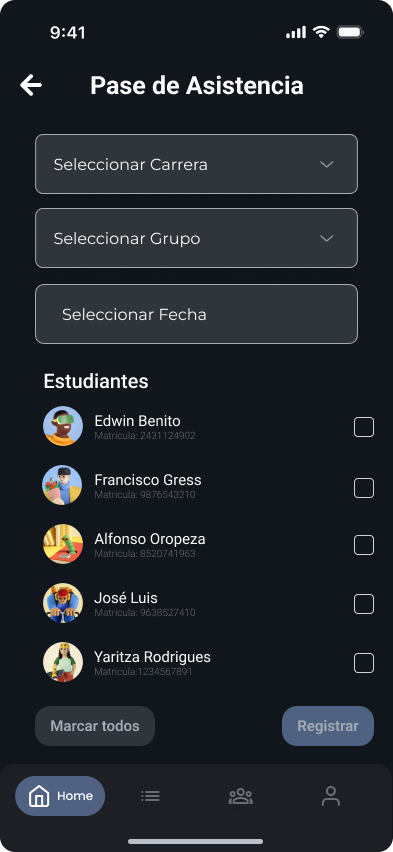
\includegraphics[width=0.22\textwidth]{./Media/Mockups/Attendance Pass.png}}{\fbox{\parbox{0.22\textwidth}{\centering Attendance Pass}}}
	\IfFileExists{./Media/Mockups/Attendance Summary.png}{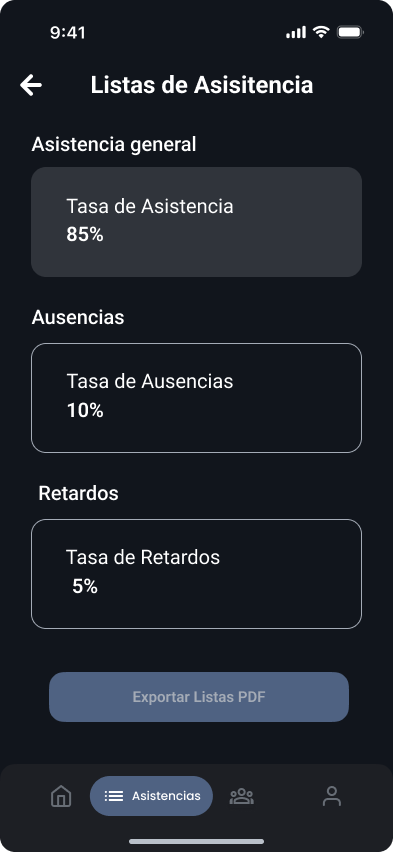
\includegraphics[width=0.22\textwidth]{./Media/Mockups/Attendance Summary.png}}{\fbox{\parbox{0.22\textwidth}{\centering Attendance Summary}}}
	\IfFileExists{./Media/Mockups/Profile Teacher.png}{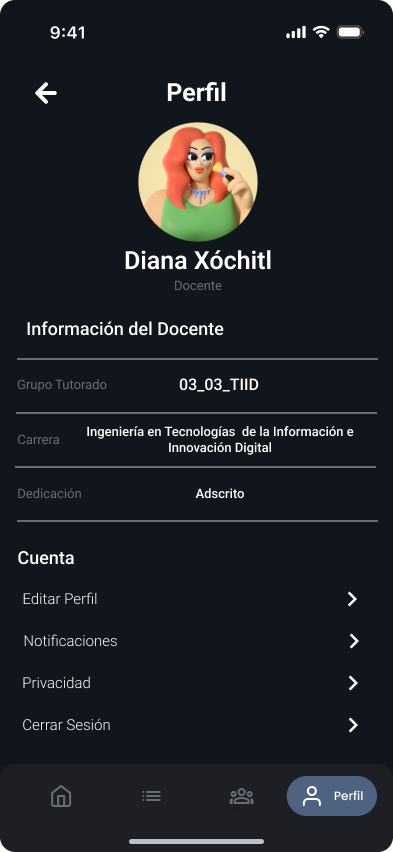
\includegraphics[width=0.22\textwidth]{./Media/Mockups/Profile Teacher.png}}{\fbox{\parbox{0.22\textwidth}{\centering Profile Teacher}}}
	\caption{Mockups del flujo del Docente: Grupos, Pase de Asistencia, Resumen y Perfil.}\label{fig:mk-teacher-flow}
\end{figure}
	\subsubsection*{Análisis de Diseño y Componentes}
	La pantalla de \textbf{Chats/Grupos} (``Chats.png'') funciona como el dashboard principal del docente, listando sus materias y el número de alumnos en cada una. La pantalla de \textbf{Pase de Asistencia} (``Attendance Pass.png'') es puramente funcional, con filtros desplegables y una lista de estudiantes con avatares y checkboxes para un registro rápido. La de \textbf{Resumen de Asistencia} (``Attendance Summary.png'') utiliza tarjetas grandes para mostrar estadísticas globales, como la tasa de asistencia, y un botón claro para exportar los datos. Finalmente, el \textbf{Perfil del Docente} (``Profile Teacher.png'') sigue la misma estructura que el del estudiante para mantener la coherencia.
    
	\subsubsection*{Flujo de Usuario y Funcionalidad}
	El docente inicia en su lista de grupos. Al seleccionar uno, podría ser dirigido al pase de asistencia. Tras registrar, puede navegar a la sección de resúmenes para ver las estadísticas consolidadas y exportar los reportes necesarios. El perfil le permite gestionar su información personal y la configuración de su cuenta.
\normalsize\end{samepage}
\clearpage

% --- Flujo de Padres de Familia ---
\subsection{ Flujo de Padres de Familia}
\begin{samepage}\small
El flujo para los padres de familia está diseñado para ser informativo y directo, proporcionando las herramientas necesarias para un seguimiento efectivo de la asistencia de sus hijos y facilitando la comunicación con la institución.
\begin{figure}[H]
	\centering
	\IfFileExists{./Media/Mockups/Child registration.png}{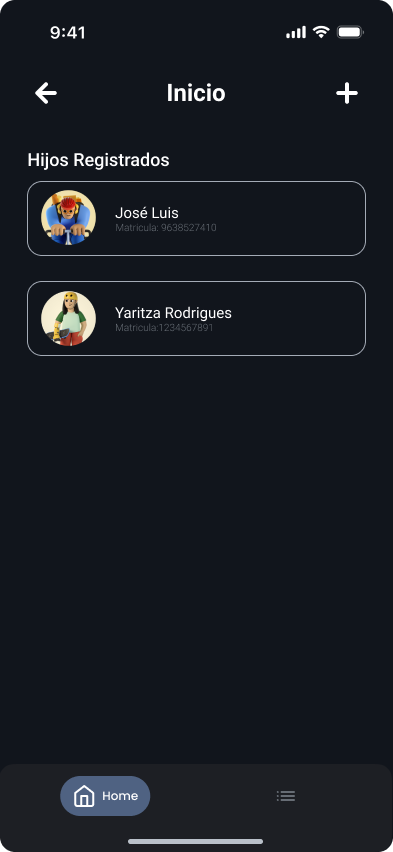
\includegraphics[width=0.22\textwidth]{./Media/Mockups/Child registration.png}}{\fbox{\parbox{0.22\textwidth}{\centering Child registration}}}
	\IfFileExists{./Media/Mockups/Attendance report.png}{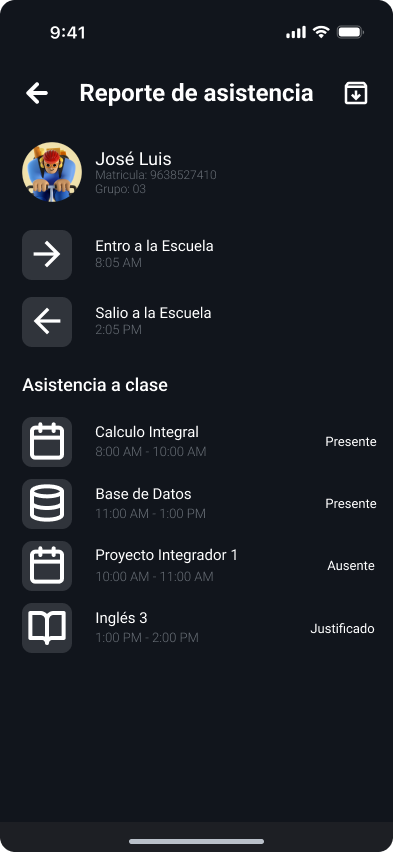
\includegraphics[width=0.22\textwidth]{./Media/Mockups/Attendance report.png}}{\fbox{\parbox{0.22\textwidth}{\centering Attendance report}}}
	\caption{Mockups del flujo de Padres de Familia: Selección de Hijo y Reporte de Asistencia.}\label{fig:mk-parents-flow}
\end{figure}
	\subsubsection*{Análisis de Diseño y Componentes}
	La pantalla de \textbf{Inicio del Padre} (``Child registration.png'') es una lista simple y clara de los ``Hijos Registrados'' bajo su tutela. Cada elemento de la lista muestra el avatar y el nombre completo del estudiante, funcionando como un punto de acceso a la información detallada. La pantalla de \textbf{Reporte de Asistencia} (``Attendance report.png'') presenta un informe diario completo para el hijo seleccionado. Destaca la información de entrada y salida de la escuela, seguida de un desglose detallado de la asistencia a cada clase del día. Un botón de descarga en la esquina superior derecha permite exportar el reporte.
    
	\subsubsection*{Flujo de Usuario y Funcionalidad}
	Al iniciar sesión, el padre ve la lista de sus hijos. Al seleccionar a uno, accede al reporte de asistencia del día actual. Desde allí, puede revisar el cumplimiento del horario escolar y el estatus en cada materia. La función de descarga le permite guardar un registro formal del día.
\normalsize\end{samepage}
\clearpage

% --- Pantalla de Carga Adicional ---
\subsection{ Pantalla de Carga}
\begin{samepage}\small
Finalmente, la pantalla de carga es un componente esencial de la experiencia de usuario que se presenta en transiciones clave. Su diseño final integra el logo de Argos, reforzando la identidad de la marca mientras el sistema procesa información en segundo plano.
\begin{figure}[H]
	\centering
	\IfFileExists{./Media/Mockups/Page Loader.png}{
\includegraphics[width=0.28\textwidth]{./Media/Mockups/Page Loader.png}}{\fbox{\parbox{0.28\textwidth}{\centering Imagen ``Page Loader.png'' no disponible}}}
	\caption{Mockup de la pantalla de carga de la aplicación.}\label{fig:mk-loader}
\end{figure}
	\subsubsection*{Análisis de Diseño y Componentes}
	El diseño es elegante y minimalista. Un círculo central oscuro contiene el isotipo de Argos en blanco, creando un punto focal. Un indicador de actividad sutil (una matriz de puntos) pulsa suavemente debajo, comunicando que la aplicación está activa sin ser visualmente abrumador. El fondo degradado añade una capa de sofisticación al diseño.
    
	\subsubsection*{Flujo de Usuario y Funcionalidad}
	Esta pantalla aparece automáticamente después de que el usuario realiza una acción que requiere tiempo de procesamiento, como iniciar sesión o generar un reporte complejo. Su función es gestionar la percepción del tiempo de espera, asegurando al usuario que su solicitud está siendo procesada y evitando que abandone la aplicación por pensar que se ha bloqueado.
\normalsize\end{samepage}

\clearpage
\section{Mapa de Navegación}

El mapa de navegación resume la arquitectura de información y los flujos de usuario de Argos. Conecta las pantallas de los mockups y define las rutas por rol para garantizar una navegación coherente e intuitiva.

\begin{samepage}\small\setlength{\parskip}{0.25\baselineskip}
\begin{figure}[H]
	\centering
	% Intentar cargar el diagrama; si no existe, mostrar un placeholder informativo de igual ancho
	\IfFileExists{./Media/MapaNavegacionpng.png}{%
		\includegraphics[width=1\textwidth]{./Media/MapaNavegacionpng.png}%
	}{%
		\IfFileExists{MapaNavegacionpng.png}{%
			\includegraphics[width=1\textwidth]{MapaNavegacionpng.png}%
		}{%
			\fbox{\parbox{0.98\textwidth}{\centering Imagen MapaNavegacionpng.png no disponible\\Coloque el archivo en ./Media/ o junto a este archivo}}% % chktex 26
		}%
	}
	\caption{Mapa de navegación de Argos por roles.}\label{fig:mapa-navegacion}
\end{figure}

\subsubsection*{Análisis del Flujo de Navegación}
\vspace{0.2\baselineskip}
Estructura jerárquica y ramificada:

\noindent \textbf{Inicio y Acceso.} Tras una posible pantalla de carga, el usuario llega a \textbf{Selección de Rol}, único punto de entrada a los tres ecosistemas.

\noindent \textbf{Ramificación por Rol.} A continuación, los tres flujos principales:
\begin{itemize}\setlength{\itemsep}{0.35em}\setlength{\parsep}{0.1em}\setlength{\parskip}{0pt}
	\item \textbf{Estudiante (Verde):} Login $\rightarrow$ Dashboard $\rightarrow$ Asistencias $\rightarrow$ Perfil.
	\item \textbf{Docente (Amarillo):} Login $\rightarrow$ Grupos/Chats $\rightarrow$ Pase de Asistencia $\rightarrow$ Resúmenes $\rightarrow$ Perfil.
	\item \textbf{Padres (Rojo):} Login $\rightarrow$ Selección de hijo $\rightarrow$ Reporte $\rightarrow$ Perfil.
\end{itemize}

\noindent \textbf{Navegación Interna.} Las flechas ``Tab'' indican saltos entre pantallas principales mediante la barra inferior (p.~ej., Dashboard $\leftrightarrow$ Perfil), sin perder contexto.

\noindent \textbf{Cierre de Ciclo.} Todos los flujos convergen en \textbf{Fin} al ``Cerrar Sesión'', regresando a Selección de Rol.

\noindent \textbf{Convenciones, Accesibilidad y Estados.} Colores por rol (verde/amarillo/rojo), iconografía y nombres de pantallas alineados con los mockups; etiquetas legibles, contraste adecuado y foco visible; se contemplan pantallas de carga y mensajes de error con rutas de retorno seguras hacia las pantallas principales.
\normalsize\end{samepage}

%%==========================================================================================%

\clearpage
\chapter{Pruebas}


\section{Pruebas de Usabilidad}

Las pruebas de usabilidad se centran en evaluar la facilidad con la que los usuarios pueden interactuar con la aplicación. Para Argos, estas pruebas se realizaron sobre los mockups de alta fidelidad para obtener retroalimentación temprana y realizar ajustes antes de la fase de desarrollo, permitiendo iterar sobre el diseño de forma ágil y con un bajo costo.

\subsection{Plan de pruebas}

Se diseñó y ejecutó un plan de pruebas de usabilidad moderadas para observar directamente cómo los usuarios representativos interactúan con los prototipos de la aplicación al realizar una serie de tareas predefinidas.

\subsubsection{Alcance de pruebas}
El alcance de estas pruebas se limitó estrictamente a la \textbf{interfaz y experiencia de usuario (UI/UX)} de los mockups interactivos de la aplicación móvil de Argos. No se evaluó el rendimiento del backend, la seguridad de la base de datos ni la infraestructura de servidores. Las pruebas se enfocaron en los siguientes aspectos:
\begin{itemize}
	\item La eficiencia y tasa de éxito en la realización de los flujos de usuario principales (pase de lista, consulta de asistencia).
	\item La claridad y comprensión de la navegación, la arquitectura de la información y la terminología utilizada.
	\item La facilidad para localizar y utilizar funciones clave dentro de cada panel de usuario.
	\item La satisfacción subjetiva del usuario al interactuar con el prototipo.
\end{itemize}

\subsubsection{Objetivos de Pruebas}
Los objetivos cuantitativos y cualitativos de las pruebas fueron los siguientes:
\begin{itemize}
	\item \textbf{Validar el flujo de pase de lista:} Medir si un docente puede registrar la asistencia de una clase de 20 alumnos en menos de 3 minutos.
	\item \textbf{Evaluar la consulta de información:} Determinar si un estudiante y un padre de familia pueden encontrar y entender el reporte de asistencia detallado en menos de 1 minuto.
	\item \textbf{Identificar puntos de fricción:} Descubrir qué elementos de la interfaz, botones o secciones generan confusión, dudas o errores en la interacción.
	\item \textbf{Recopilar retroalimentación cualitativa:} Obtener opiniones, comentarios y sugerencias directas de los usuarios para mejorar la experiencia general de la aplicación.
\end{itemize}

\clearpage
\subsubsection{Entorno de pruebas}
Las pruebas se llevaron a cabo en un entorno controlado y neutral (un aula vacía en la UPP) para minimizar distracciones y simular un contexto de uso realista. Cada sesión individual contó con:
\begin{itemize}
	\item \textbf{Un participante:} Un usuario final real (estudiante, docente o padre de familia).
	\item \textbf{Un dispositivo móvil:} Un smartphone con el prototipo interactivo de los mockups cargado.
	\item \textbf{Un moderador:} Encargado de guiar la sesión, asignar las tareas y realizar preguntas.
	\item \textbf{Un observador:} Responsable de tomar notas detalladas sobre el comportamiento, las acciones y los comentarios del usuario.
\end{itemize}

\subsubsection{Resultados y/o Hallazgos}

Tras la ejecución de las pruebas con 5 participantes por cada rol, se consolidaron los siguientes hallazgos:

\begin{itemize}
    \item \textbf{Hallazgo 1 (Positivo):} El 85\% de los docentes participantes completaron la tarea de pase de lista dentro del tiempo objetivo, calificando el flujo como ``muy intuitivo y rápido''.
    \item \textbf{Hallazgo 2 (Mejora):} El 30\% de los estudiantes tardaron más de lo esperado en encontrar la opción para descargar su historial, sugiriendo que el botón podría tener una ubicación más prominente o un texto más claro.
    \item \textbf{Hallazgo 3 (Sugerencia):} El 60\% de los padres de familia sugirieron que la gráfica de asistencia en su panel debería permitir un filtro por semana, además del filtro mensual, para un seguimiento más granular.
    \item \textbf{Hallazgo 4 (Positivo):} El 85\% de los participantes comprendieron y utilizaron correctamente la navegación principal a través de la barra de pestañas inferior sin necesidad de guía, validando la arquitectura de la información.
\end{itemize}

\subsubsection*{Encuesta de Usabilidad y Experiencia de Usuario}

Con el objetivo de evaluar la usabilidad, accesibilidad y efectividad de las principales funciones de la plataforma, se aplicó una encuesta a tres grupos de usuarios: docentes, estudiantes y padres de familia.  

La encuesta se centró en identificar:
\begin{itemize}
    \item El nivel de facilidad para completar tareas clave (pase de lista, descarga de historial académico y navegación general).
    \item El grado de satisfacción con la experiencia de uso.
    \item Las principales sugerencias de mejora para optimizar la interacción con la plataforma.
\end{itemize}

Los resultados obtenidos permiten identificar fortalezas en la arquitectura de la información y áreas de oportunidad en la visibilidad de ciertas funciones, así como nuevas necesidades expresadas por los usuarios.



% Docentes y Estudiantes (fila 1)
\begin{figure}[H]
    \centering
    \begin{minipage}[b]{0.50\textwidth}
        \centering
        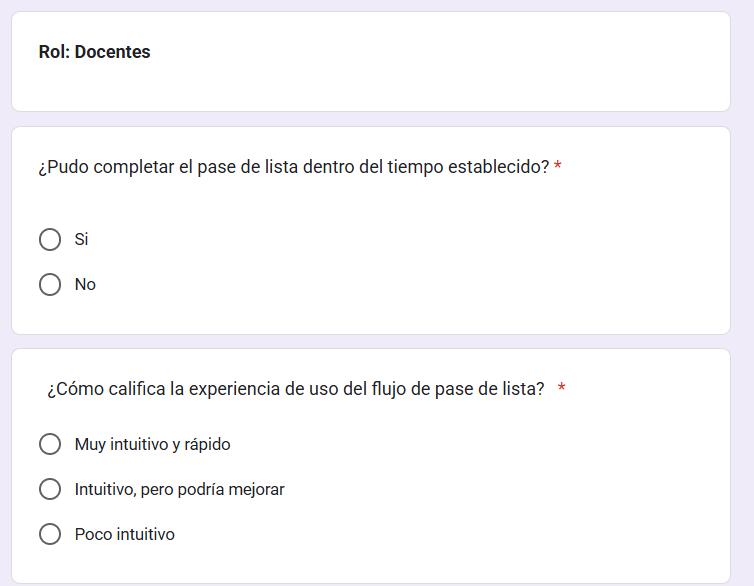
\includegraphics[width=1.0\textwidth]{./Media/p1.png}
        \caption{Encuesta aplicada a docentes.}
    \end{minipage}

    \begin{minipage}[b]{0.50\textwidth}
        \centering
        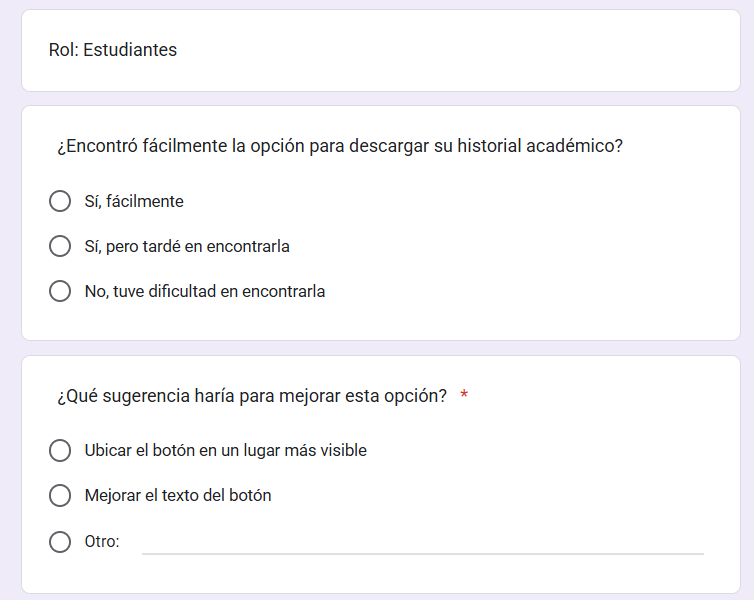
\includegraphics[width=1.0\textwidth]{./Media/p2.png}
        \caption{Encuesta aplicada a estudiantes.}
    \end{minipage}

     \centering
    \begin{minipage}[b]{0.50\textwidth}
        \centering
        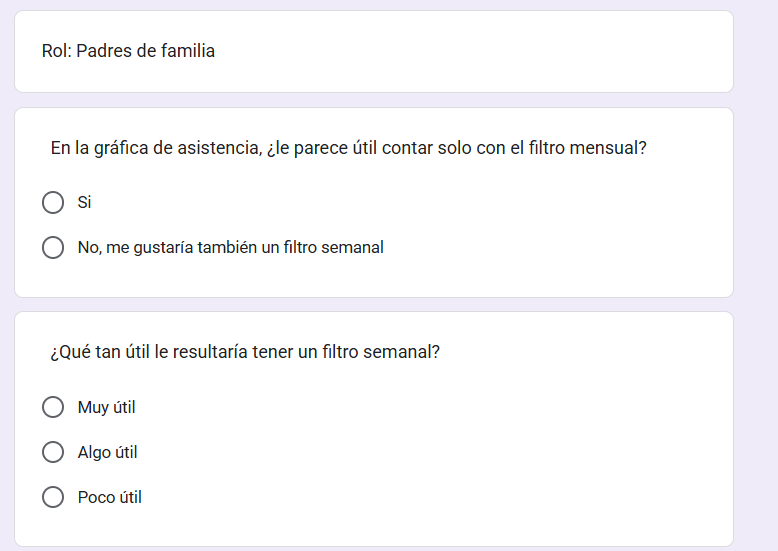
\includegraphics[width=1.0\textwidth]{./Media/p3.png}
        \caption{Encuesta aplicada a padres de familia.}
    \end{minipage}

\end{figure}


% Circulo (fila 3)
\begin{figure}[H]
    \centering
    \begin{minipage}[b]{0.65\textwidth}
        \centering
        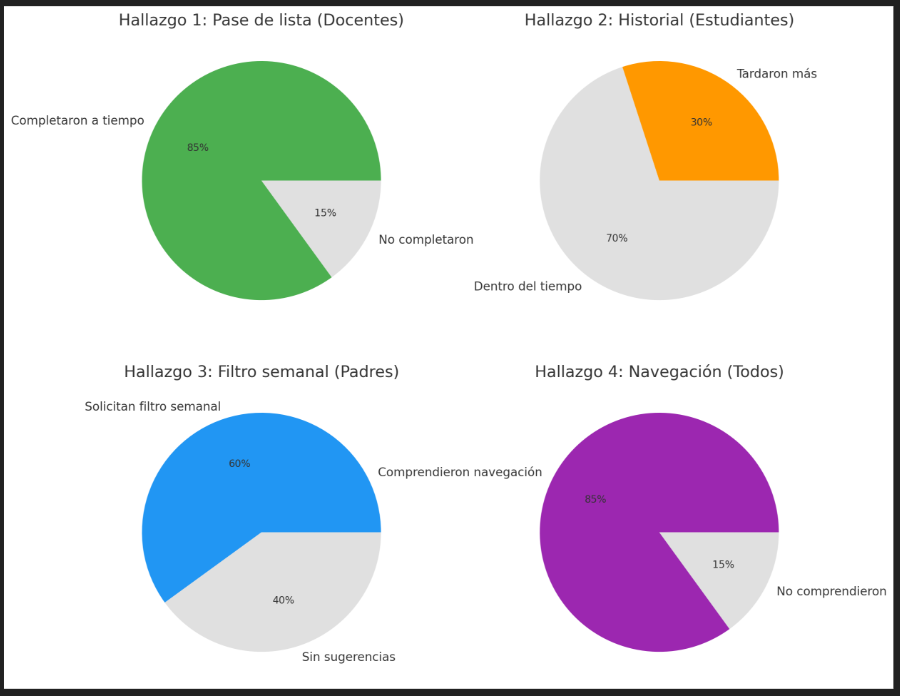
\includegraphics[width=1.0\textwidth]{./Media/Circulo.png}
        \caption{Gráfica comparativa circular de los hallazgos obtenidos en la encuesta.}
    \end{minipage}

     \centering
    \begin{minipage}[b]{0.65\textwidth}
        \centering
        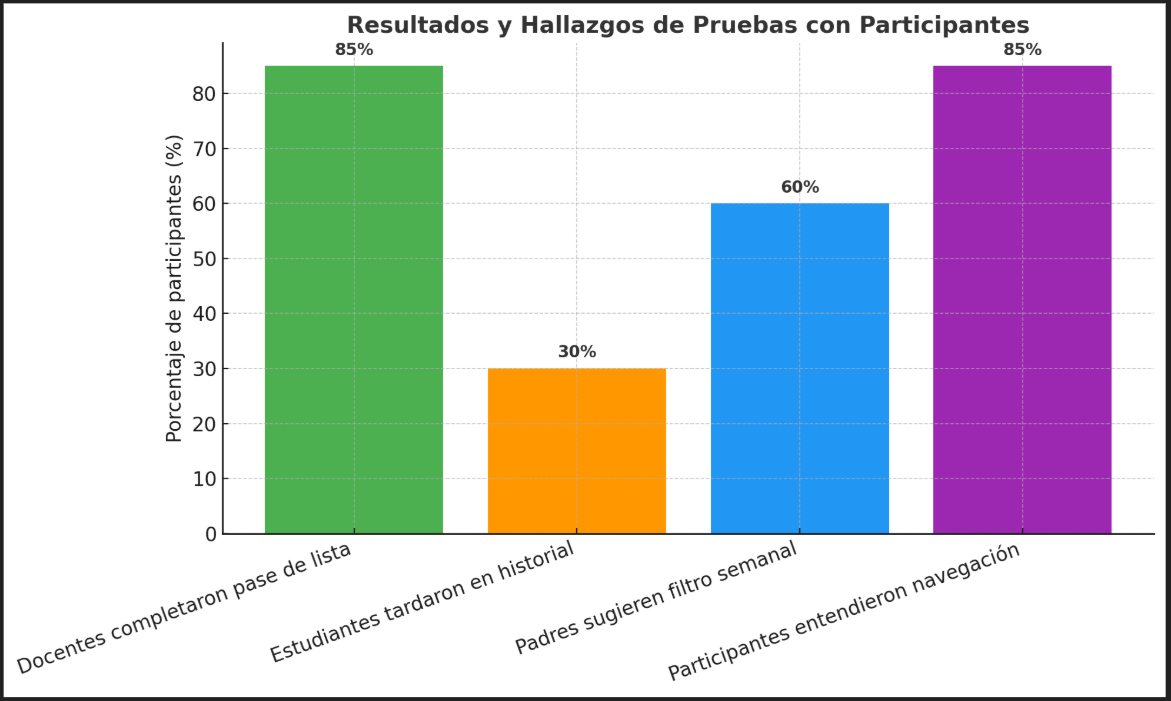
\includegraphics[width=1.0\textwidth]{./Media/Barras.png}
        \caption{Gráfica comparativa de barras de los hallazgos obtenidos en la encuesta.}
    \end{minipage}
\end{figure}


\subsubsection{Conclusión Final}
Las pruebas de usabilidad concluyeron que los flujos de trabajo principales de la aplicación Argos son sólidos, eficientes y fáciles de seguir para todos los roles de usuario. Los hallazgos permitieron identificar oportunidades de mejora específicas y de alto valor, principalmente en la visibilidad de funciones secundarias y en la flexibilidad de los filtros de datos. Las recomendaciones, como rediseñar la ubicación del botón de descarga y añadir un filtro semanal en el panel de padres, serán incorporadas en la siguiente iteración del diseño antes de proceder con el desarrollo.

\clearpage
\section{Pruebas de Proyecto}

Las pruebas de proyecto van más allá de la interfaz y buscan validar el concepto, la estrategia y la viabilidad de la iniciativa Argos en el contexto institucional, asegurando su alineación con las necesidades y capacidades de la universidad.

\subsection{Focus Group con Especialistas}

\subsubsection{Definición}
Un focus group es una técnica de investigación cualitativa que reúne a un pequeño grupo de expertos (entre 3 y 5 personas) para discutir un tema específico bajo la guía de un moderador. A diferencia de una entrevista, fomenta la interacción y el debate entre los participantes.

\subsubsection{Objetivo}
Para el Proyecto Argos, se organizó un focus group con especialistas clave de la UPP (un coordinador académico, el jefe de servicios de TI y un administrador escolar). El objetivo fue \textbf{presentar el proyecto en su totalidad (problema, solución, mockups, plan) y validar su viabilidad técnica, operativa y estratégica} desde una perspectiva institucional, recogiendo su feedback experto.

\subsubsection{Ventajas}
Realizar esta prueba de concepto con especialistas aportó beneficios estratégicos:
\begin{itemize}
	\item \textbf{Identificación Temprana de Riesgos:} Los especialistas ayudaron a identificar posibles desafíos de integración con los sistemas escolares existentes (como Banner) y con las políticas de seguridad de la red universitaria.
	\item \textbf{Obtención de Apoyo (Buy-in):} Presentar el proyecto y tomar en cuenta sus opiniones generó apoyo temprano de figuras clave, lo cual es vital para la futura implementación del proyecto.
	\item \textbf{Sugerencias de Expertos:} Se obtuvieron valiosas recomendaciones sobre normativas de protección de datos que la universidad debe seguir, así como ideas para una posible implementación piloto en un solo departamento.
\end{itemize}

\clearpage
\subsection{Adaptación de Innovaciones}

\subsubsection{Definición}
La adaptación de innovaciones es el proceso de analizar y planificar cómo una nueva tecnología o sistema será adoptado por una comunidad. Se enfoca en comprender y gestionar los factores sociales, culturales y psicológicos que influyen en la aceptación del cambio para asegurar una transición exitosa.

\subsubsection{Objetivo}
El objetivo para Argos es \textbf{diseñar una estrategia proactiva que asegure una transición suave y una alta tasa de adopción} del nuevo sistema por parte de toda la comunidad universitaria. Esto incluye planificar cómo se comunicarán los beneficios, cómo se abordarán las preocupaciones sobre privacidad (especialmente con el reconocimiento facial), y cómo se diseñarán los programas de capacitación para los diferentes roles.

\subsubsection{Ventajas}
Planificar la adaptación de la innovación desde la fase de diseño ofrece ventajas a largo plazo:
\begin{itemize}
	\item \textbf{Reduce la Resistencia al Cambio:} Al anticipar y abordar las preocupaciones de los usuarios (ej. "¿Qué pasará con mis datos biométricos?"), se minimiza la fricción y la oposición durante la implementación.
	\item \textbf{Asegura el Retorno de Inversión (ROI):} Una alta tasa de adopción por parte de los usuarios finales es la única manera de garantizar que los beneficios proyectados del sistema (eficiencia, seguridad, datos precisos) se materialicen.
	\item \textbf{Construye Confianza y Transparencia:} Una comunicación clara y una buena capacitación generan confianza en la nueva tecnología y en la gestión de la institución, demostrando que se toma en cuenta el factor humano.
\end{itemize}



\backmatter
% bibliography, glossary and index would go here.

\end{document}